%%%%%%%%%%%%%%%%%%%%%%%%%%%%%%%%%%%%%%%%
% datoteka analiza_in_predstavitev_podatkov_iz_hladne_verige.tex
%



\documentclass[a4paper, 12pt]{book}
%\documentclass[a4paper, 12pt, draft]{book}  Nalogo preverite tudi z opcijo draft, ki vam bo pokazala, katere vrstice so predolge!



\usepackage[utf8x]{inputenc}   % omogoča uporabo slovenskih črk kodiranih v formatu UTF-8
\usepackage[slovene,english]{babel}    % naloži, med drugim, slovenske delilne vzorce
\usepackage[pdftex]{graphicx}  % omogoča vlaganje slik različnih formatov
\usepackage{fancyhdr}          % poskrbi, na primer, za glave strani
\usepackage{amssymb}           % dodatni simboli
\usepackage{amsmath}           % eqref, npr.
%\usepackage{hyperxmp}
\usepackage[hyphens]{url}  % dodal Solina
\usepackage{comment}       % dodal Solina

\usepackage[pdftex, colorlinks=true,
						citecolor=black, filecolor=black, 
						linkcolor=black, urlcolor=black,
						pagebackref=false, 
						pdfproducer={LaTeX}, pdfcreator={LaTeX}, hidelinks]{hyperref}

\usepackage{color}       % dodal Solina
\usepackage{soul}       % dodal Solina


%%%%%%%%%%%%%%%%%%%%%%%%%%%%%%%%%%%%%%%%
%	CUSTOME
%%%%%%%%%%%%%%%%%%%%%%%%%%%%%%%%%%%%%%%%
\usepackage{array}
\usepackage{tabularx}
\usepackage{listings}
\usepackage{xcolor}


\renewcommand{\lstlistingname}{Koda}
\renewcommand{\lstlistlistingname}{Seznam kod}

\newcolumntype{b}{X}
\newcolumntype{s}{>{\hsize=.9\hsize}X}
\newcolumntype{z}{>{\hsize=.2\hsize}X}

\definecolor{codegreen}{rgb}{0,0.6,0}
\definecolor{codegray}{rgb}{0.5,0.5,0.5}
\definecolor{codepurple}{rgb}{0.58,0,0.82}
\definecolor{backcolour}{rgb}{0.95,0.95,0.92}

\lstdefinestyle{mystyle}{
    backgroundcolor=\color{backcolour},   
    commentstyle=\color{codegreen},
    keywordstyle=\color{magenta},
    numberstyle=\tiny\color{codegray},
    stringstyle=\color{codepurple},
    basicstyle=\ttfamily\footnotesize,
    breakatwhitespace=false,         
    breaklines=true,                 
    captionpos=b,                    
    keepspaces=true,                 
    numbers=left,                    
    numbersep=5pt,                  
    showspaces=false,                
    showstringspaces=false,
    showtabs=false,                  
    tabsize=2
}

%%%%%%%%%%%%%%%%%%%%%%%%%%%%%%%%%%%%%%%%
%	DIPLOMA INFO
%%%%%%%%%%%%%%%%%%%%%%%%%%%%%%%%%%%%%%%%
\newcommand{\ttitle}{Analiza in predstavitev podatkov iz hladne verige}
\newcommand{\ttitleEn}{Analysis and presentation of cold chain data}
\newcommand{\tsubject}{\ttitle}
\newcommand{\tsubjectEn}{\ttitleEn}
\newcommand{\tauthor}{Andraž Hostnik}
\newcommand{\tkeywords}{hladna veriga, doba uporabnosti, spletna aplikcija, Laravel}
\newcommand{\tkeywordsEn}{cold chain, shelf life, web application, Laravel}


%%%%%%%%%%%%%%%%%%%%%%%%%%%%%%%%%%%%%%%%
%	HYPERREF SETUP
%%%%%%%%%%%%%%%%%%%%%%%%%%%%%%%%%%%%%%%%
\hypersetup{pdftitle={\ttitle}}
\hypersetup{pdfsubject=\ttitleEn}
\hypersetup{pdfauthor={\tauthor, ah0699@student.uni-lj.si}}
\hypersetup{pdfkeywords=\tkeywordsEn}


 


%%%%%%%%%%%%%%%%%%%%%%%%%%%%%%%%%%%%%%%%
% postavitev strani
%%%%%%%%%%%%%%%%%%%%%%%%%%%%%%%%%%%%%%%%  

\addtolength{\marginparwidth}{-20pt} % robovi za tisk
\addtolength{\oddsidemargin}{40pt}
\addtolength{\evensidemargin}{-40pt}

\renewcommand{\baselinestretch}{1.3} % ustrezen razmik med vrsticami
\setlength{\headheight}{15pt}        % potreben prostor na vrhu
\renewcommand{\chaptermark}[1]%
{\markboth{\MakeUppercase{\thechapter.\ #1}}{}} \renewcommand{\sectionmark}[1]%
{\markright{\MakeUppercase{\thesection.\ #1}}} \renewcommand{\headrulewidth}{0.5pt} \renewcommand{\footrulewidth}{0pt}
\fancyhf{}
\fancyhead[LE,RO]{\sl \thepage} 
\fancyhead[LO]{\sl \rightmark} \fancyhead[RE]{\sl \leftmark}
%\fancyhead[RE]{\sc \tauthor}              % dodal Solina
%\fancyhead[LO]{\sc Diplomska naloga}     % dodal Solina


\newcommand{\BibTeX}{{\sc Bib}\TeX}

%%%%%%%%%%%%%%%%%%%%%%%%%%%%%%%%%%%%%%%%
% naslovi
%%%%%%%%%%%%%%%%%%%%%%%%%%%%%%%%%%%%%%%%  


\newcommand{\autfont}{\Large}
\newcommand{\titfont}{\LARGE\bf}
\newcommand{\clearemptydoublepage}{\newpage{\pagestyle{empty}\cleardoublepage}}
\setcounter{tocdepth}{1}	      % globina kazala

%%%%%%%%%%%%%%%%%%%%%%%%%%%%%%%%%%%%%%%%
% konstrukti
%%%%%%%%%%%%%%%%%%%%%%%%%%%%%%%%%%%%%%%%  
\newtheorem{izrek}{Izrek}[chapter]
\newtheorem{trditev}{Trditev}[izrek]
\newenvironment{dokaz}{\emph{Dokaz.}\ }{\hspace{\fill}{$\Box$}}

%%%%%%%%%%%%%%%%%%%%%%%%%%%%%%%%%%%%%%%%%%%%%%%%%%%%%%%%%%%%%%%%%%%%%%%%%%%%%%%
%% PDF-A
%%%%%%%%%%%%%%%%%%%%%%%%%%%%%%%%%%%%%%%%%%%%%%%%%%%%%%%%%%%%%%%%%%%%%%%%%%%%%%%


%%%%%%%%%%%%%%%%%%%%%%%%%%%%%%%%%%%%%%%% 
% define medatata
%%%%%%%%%%%%%%%%%%%%%%%%%%%%%%%%%%%%%%%% 
\def\Title{\ttitle}
\def\Author{\tauthor, ah0699@student.uni-lj.si}
\def\Subject{\ttitleEn}
\def\Keywords{\tkeywordsEn}

%%%%%%%%%%%%%%%%%%%%%%%%%%%%%%%%%%%%%%%% 
% \convertDate converts D:20080419103507+02'00' to 2008-04-19T10:35:07+02:00
%%%%%%%%%%%%%%%%%%%%%%%%%%%%%%%%%%%%%%%% 
\def\convertDate{%
    \getYear
}

{\catcode`\D=12
 \gdef\getYear D:#1#2#3#4{\edef\xYear{#1#2#3#4}\getMonth}
}
\def\getMonth#1#2{\edef\xMonth{#1#2}\getDay}
\def\getDay#1#2{\edef\xDay{#1#2}\getHour}
\def\getHour#1#2{\edef\xHour{#1#2}\getMin}
\def\getMin#1#2{\edef\xMin{#1#2}\getSec}
\def\getSec#1#2{\edef\xSec{#1#2}\getTZh}
\def\getTZh +#1#2{\edef\xTZh{#1#2}\getTZm}
\def\getTZm '#1#2'{%
    \edef\xTZm{#1#2}%
    \edef\convDate{\xYear-\xMonth-\xDay T\xHour:\xMin:\xSec+\xTZh:\xTZm}%
}

\expandafter\convertDate\pdfcreationdate 

%%%%%%%%%%%%%%%%%%%%%%%%%%%%%%%%%%%%%%%%
% get pdftex version string
%%%%%%%%%%%%%%%%%%%%%%%%%%%%%%%%%%%%%%%% 
\newcount\countA
\countA=\pdftexversion
\advance \countA by -100
\def\pdftexVersionStr{pdfTeX-1.\the\countA.\pdftexrevision}


%%%%%%%%%%%%%%%%%%%%%%%%%%%%%%%%%%%%%%%%
% XMP data
%%%%%%%%%%%%%%%%%%%%%%%%%%%%%%%%%%%%%%%%  
\usepackage{xmpincl}
\includexmp{pdfa-1b}

%%%%%%%%%%%%%%%%%%%%%%%%%%%%%%%%%%%%%%%%
% pdfInfo
%%%%%%%%%%%%%%%%%%%%%%%%%%%%%%%%%%%%%%%%  
\pdfinfo{%
    /Title    (\ttitle)
    /Author   (\tauthor, ah0699@student.uni-lj.si)
    /Subject  (\ttitleEn)
    /Keywords (\tkeywordsEn)
    /ModDate  (\pdfcreationdate)
    /Trapped  /False
}

% list

\newenvironment{myitemize}
{ \begin{itemize}
    \setlength{\itemsep}{2pt}
    \setlength{\parskip}{0pt}
    \setlength{\parsep}{2pt}     }
{ \end{itemize}                  } 


%%%%%%%%%%%%%%%%%%%%%%%%%%%%%%%%%%%%%%%%%%%%%%%%%%%%%%%%%%%%%%%%%%%%%%%%%%%%%%%
%%%%%%%%%%%%%%%%%%%%%%%%%%%%%%%%%%%%%%%%%%%%%%%%%%%%%%%%%%%%%%%%%%%%%%%%%%%%%%%
\begin{document}
\selectlanguage{slovene}
\frontmatter
\setcounter{page}{1} %
\renewcommand{\thepage}{}       % preprecimo težave s številkami strani v kazalu
\newcommand{\sn}[1]{"`#1"'}                    % dodal Solina (slovenski narekovaji)

%%%%%%%%%%%%%%%%%%%%%%%%%%%%%%%%%%%%%%%%
%naslovnica
 \thispagestyle{empty}%
   \begin{center}
    {\large\sc Univerza v Ljubljani\\%
      Fakulteta za računalništvo in informatiko}%
    \vskip 10em%
    {\autfont \tauthor\par}%
    {\titfont \ttitle \par}%
    {\vskip 3em \textsc{DIPLOMSKO DELO\\[5mm]         % dodal Solina za ostale študijske programe
    VISOKOŠOLSKI STROKOVNI ŠTUDIJSKI PROGRAM\\ PRVE STOPNJE\\ RAČUNALNIŠTVO IN INFORMATIKA}\par}%
%   UNIVERZITETNI  ŠTUDIJSKI PROGRAM\\ PRVE STOPNJE\\ RAČUNALNIŠTVO IN INFORMATIKA}\par}%
%    INTERDISCIPLINARNI UNIVERZITETNI\\ ŠTUDIJSKI PROGRAM PRVE STOPNJE\\ RAČUNALNIŠTVO IN MATEMATIKA}\par}%
%    INTERDISCIPLINARNI UNIVERZITETNI\\ ŠTUDIJSKI PROGRAM PRVE STOPNJE\\ UPRAVNA INFORMATIKA}\par}%
%    INTERDISCIPLINARNI UNIVERZITETNI\\ ŠTUDIJSKI PROGRAM PRVE STOPNJE\\ MULTIMEDIJA}\par}%
    \vfill\null%
    {\large \textsc{Mentor}: doc.\ dr.  Mira Trebar\par}%
%   {\large \textsc{Somentor}:  izr.\ prof.\ dr. Martin Krpan \par}%
    {\vskip 2em \large Ljubljana, 2020 \par}%
\end{center}
% prazna stran
%\clearemptydoublepage      % dodal Solina (izjava o licencah itd. se izpiše na hrbtni strani naslovnice)

%%%%%%%%%%%%%%%%%%%%%%%%%%%%%%%%%%%%%%%%
%copyright stran
\thispagestyle{empty}
\vspace*{8cm}

\noindent
{\sc Copyright}. 
Rezultati diplomske naloge so intelektualna lastnina avtorja in Fakultete za računalništvo in informatiko Univerze v Ljubljani.
Za objavo in koriščenje rezultatov diplomske naloge je potrebno pisno privoljenje avtorja, Fakultete za računalništvo in informatiko ter mentorja.

\begin{center}
\mbox{}\vfill
\emph{Besedilo je oblikovano z urejevalnikom besedil \LaTeX.}
\end{center}
% prazna stran
\clearemptydoublepage

%%%%%%%%%%%%%%%%%%%%%%%%%%%%%%%%%%%%%%%%
% stran 3 med uvodnimi listi
\thispagestyle{empty}
\vspace*{4cm}

\noindent
Fakulteta za računalništvo in informatiko izdaja naslednjo nalogo:
\medskip
\begin{tabbing}
\hspace{32mm}\= \hspace{6cm} \= \kill




Tematika naloge:
\end{tabbing}
Temperatura in vlaga sta pomembna parametra v nadzoru hladne verige hitro pokvarljivih živil. Z uporabo samostojnih merilnih naprav ali različnih senzorskih sistemov so pridobljeni podatki pogosto na voljo v obliki zapisov v datotekah. Kandidat naj v diplomskem delu izdela spletno aplikacijo za vnos, obdelavo in prikaz izmerjenih temperatur in relativne vlage. Podatke naj  analizira in uporabi za izračun preostale dobe uporabnosti ter rezultate predstavi v časovnem grafu. Pomembne ugotovitve naj predstavi tudi z enostavnim načinom obveščanja v tekstovni obliki. Rešitev naj omogoča dva tipa uporabnikov, za urejanje ali pregled. Izdelana naj bo z uporabo ogrodja Laravel, sodobnih spletnih tehnologij in podatkovno bazo MySQL. Implementacija in testiranje naj vključujeta predstavitev rezultatov z realnimi meritvami hladne verige. 
\vspace{15mm}






\vspace{2cm}

% prazna stran
\clearemptydoublepage

% zahvala
\thispagestyle{empty}\mbox{}\vfill\null\it%
\noindent
Zahvaljujem se mentorici doc. dr. Miri Trebar za vso pomoč in nasvete pri izdelavi diplomske naloge. Posebna zahvala gre tudi moji družini.
\rm\normalfont

% prazna stran
\clearemptydoublepage


%%%%%%%%%%%%%%%%%%%%%%%%%%%%%%%%%%%%%%%%
% kazalo
\pagestyle{empty}
\def\thepage{}% preprecimo tezave s stevilkami strani v kazalu
\tableofcontents{}


% tole naj bi mi kao clearalo empty page pa mi ne !
\let\cleardoublepage=\clearpage

%%%%%%%%%%%%%%%%%%%%%%%%%%%%%%%%%%%%%%%%
% seznam kratic

\chapter*{Seznam uporabljenih kratic}  % spremenil Solina, da predolge vrstice ne gredo preko desnega roba
\noindent\begin{tabular}{p{0.2\textwidth}|p{.35\textwidth}|p{.35\textwidth}}    % po potrebi razširi prvo kolono tabele na račun drugih dveh!
  {\bf kratica} & {\bf angleško}                             & {\bf slovensko} \\ \hline
%  {\bf API} & Application Programming Interface & aplikacijski programski vmesnik \\
  {\bf CSIRO} & Commonwealth Scientic and Industrial Research Organisation & Commonwealth Scientic and Industrial Research Organisation \\
  {\bf CSS} & Cascading Style Sheets & predloge, ki določajo izgled spletnih strani \\
  {\bf CSV} & Comma Separated Values & podatki so v datoteki ločeni z vejico \\
  {\bf ER diagram} & Entity Relationship Diagram & entitetno relacijski diagram \\
  {\bf FTP} & File Transfer Protocol & protokol za prenos datotek \\
  {\bf HTML} & Hyper Text Markup Language & označevalni jezik za izdelavo spletnih strani \\
  {\bf HTTP} & Hyper Text Transfer Protocol & komunikacijski spletni protokol \\
%  {\bf FTP} & File Transfer Protocol & protokol za prenos datotek \\
%  {\bf IAAA} & Identification, Authentication, Authorization and Accounting & varnostni koncepti: identifikacija, avtentikacija, avtorizacija in odgovornost \\
%  {\bf JSON} & JavaScript Object Notation & objektna notacija za JavaScript \\
  {\bf MVC} & Model--view--controller & model--pogled--krmilnik \\
  {\bf NFC} & Near Field Communication & tehnologija komunikacije kratkega dosega \\
  {\bf PDF} & Portable Document Format & format prenosnega dokumenta \\
  {\bf PHP} & Personal Home Page (PHP: Hypertext Preprocessor) & skriptni programski jezik \\
  {\bf REST} & Representational state transfer & predstavitveni prenos stanja \\
%  {\bf SAL} & ??? & ??? \\
%  {\bf SL} 	& Shelf Life & doba uporabnosti \\
%  {\bf SQL} & Structured Query Language & strukturiran poizvedovalni jezik \\
  {\bf URL} & Uniform Resource Locator & enolični krajevnik vira \\
%  \dots & \dots & \dots \\
\end{tabular}


% prazna stran
\clearemptydoublepage

%%%%%%%%%%%%%%%%%%%%%%%%%%%%%%%%%%%%%%%%
% povzetek
\addcontentsline{toc}{chapter}{Povzetek}
\chapter*{Povzetek}

\noindent\textbf{Naslov:} \ttitle
\bigskip

\noindent\textbf{Avtor:} \tauthor
\bigskip

%\noindent\textbf{Povzetek:} 
\noindent
V današnjem svetu igrajo podatki zelo pomembno vlogo v nadzoru hladne verige hitro pokvarljivih živil. Običajno prihajajo iz različnih senzorskih sistemov in v različnih podatkovnih formatih, pogosto pa se zbirajo in shranjujejo tudi v datotekah. Za takšen primer smo razvili spletno aplikacijo, ki omogoča enostaven vnos, shranjevanje, analizo in vizualizacijo celotnega postopka zajema senzorskih meritev.  Omogočeno je dodajanje in urejanje parametrov, ki so povezani z meritvami. Na podlagi vnaprej definiranih zahtev o ravnanju z živili v hladni verigi in z analizo meritev se izračuna preostala doba uporabnosti, ki je prikazana v časovnem grafu. V aplikaciji so nazorno prikazane tudi morebitne anomalije v podatkih. V diplomski nalogi je opisan postopek izdelave spletne aplikacije, ki smo jo razvijali z ogrodjem Laravel in podatkovno bazo MySQL. Grafični vmesnik je prilagojen za vse vrste naprav, za potrebe lažjega testiranja je bil dodan tudi generator podatkov, ki omogoča dodatne analize simuliranih dogodkov v hladni verigi. Vključeno je dodeljevanje in urejanje pravic uporabnikov. Na koncu smo spletno aplikacijo testirali z realnimi meritvami hladne verige.
\bigskip

\noindent\textbf{Ključne besede:} \tkeywords.
% prazna stran
\clearemptydoublepage

%%%%%%%%%%%%%%%%%%%%%%%%%%%%%%%%%%%%%%%%
% abstract
\selectlanguage{english}
\addcontentsline{toc}{chapter}{Abstract}
\chapter*{Abstract}

\noindent\textbf{Title:} \ttitleEn
\bigskip

\noindent\textbf{Author:} \tauthor
\bigskip

%\noindent\textbf{Abstract:} 
\noindent TODO english abstract from uvod.
\bigskip

\noindent\textbf{Keywords:} \tkeywordsEn.
\selectlanguage{slovene}
% prazna stran
\clearemptydoublepage

%%%%%%%%%%%%%%%%%%%%%%%%%%%%%%%%%%%%%%%%
\mainmatter
\setcounter{page}{1}
\pagestyle{fancy}

\chapter{Uvod}
Kakovostna in varna hrana predstavlja vse večji izziv tako na lokalnem, kot tudi globalnem trgu proizvodnje in distribucije. Potrošniki postajajo bolj osveščeni in pričakujejo vse več informacij o prehranski verigi živil, ki ne predstavlja tveganj za njihovo zdravje. Iz tega razloga so zelo pomembni podatki iz hladne verige, ki so pridobljeni v vseh fazah, od začetka priprave proizvoda za prodajo in vse do prodajnega mesta, kjer so na voljo končnim uporabnikom. Pri zagotavljanju hladne verige živil gre lahko marsikaj narobe, zato sistemi za zajem podatkov in aplikacije za analizo in vizualizacijo tovrstnih podatkov odigrajo ključno vlogo pri ugotavljanju in odpravljanju težav ali napak.

Podatki, ki zagotavljajo meritve v celotni hladni verigi, običajno prihajajo iz različnih senzorskih sistemov in v različnih podatkovnih formatih. Na področju analize in prikaza podatkov iz hladne verige obstaja že kar nekaj senzorskih sistemov, ki so sestavni del interneta stvari v prehranskih verigah. Še vedno pa se pogosto zbirajo in shranjujejo v datotekah, kjer so zapisani tudi v različnih podatkovnih formatih in  niso avtomatsko na voljo v spletnih aplikacijah. Njihovo analizo je nato mogoče izvesti z ročno obdelavo podatkov v ustreznih programskih orodjih, kar pa ne rešuje problema enostavnega in preglednega informiranja o morebitnih težavah, ki so pomembne za določanje preostale dobe uporabnosti hitro pokvarljivih živil. Zaradi izpostavljenosti višjim temperaturam je živilo še vedno primerno za uživanje, se je pa skrajšal čas v katerem ga je potrebno porabiti. 

V ta namen smo se odločili razviti enotno spletno aplikacijo, ki omogoča enostaven vnos in shranjevanje vhodnih podatkov, analizo in vizualizacijo celotnega postopka zajema senzorskih meritev. Na podlagi vnaprej definiranih zahtev o ravnanju z živili v hladni verigi in z analizo meritev in izbranih metod je možno določiti preostalo dobo uporabnosti. Aplikacija nazorno prikaže tudi anomalije v podatkih in tako opozori na morebitne napake ali pomanjkljivosti v procesu hladne verige ali delovanja senzorskega sistema.

Aplikacija je razvita s sodobnimi spletnimi orodji in tehnologijami, prilagojena za vse vrste naprav in enostavna za uporabo. Za potrebe lažjega testiranja smo razvili tudi generator podatkov, ki omogoča dodatne analize simuliranih dogodkov v hladni verigi. Poleg tega vsebuje tudi dodajanje in urejanje posameznih parametrov ter dodeljevanje in urejanje pravic uporabnikov.

V diplomski nalogi najprej opišemo senzorske podatke s katerimi razpolagamo v aplikaciji. V drugem poglavju na kratko opišemo uporabljena orodja in tehnologije pri izdelavi spletne aplikacije. Sledi poglavje o predstavitvi funkcionalnih in nefunkcionalnih zahtev, podatkovnem modelu, načrtu arhitekture in opisu zaslonskih predlogov. V četrtem poglavju je podrobno predstavljen potek implementacije spletne rešitve z zaslonskimi slikami. Na koncu sledita še opis postopka testiranja in sklepne ugotovitve.



\chapter{Pregled področja}
\label{pregled-podrocja}

V poglavju na kratko predstavimo hladno verigo, obstoječe spletne rešitve in opišemo senzorske podatke, ki so uporabljeni v diplomski nalogi.

\section{Hladna veriga}

Zahteve potrošnikov po raznoliki in kvalitetni hrani se iz leta v leto povečujejo, s tem pa se povečujejo tudi zahteve po prevozu in shranjevanju ohlajenih in zmrzjenih živil. Živila lahko potujejo preko celega planeta, preden pridejo do končnega uporabnika. Čez celoten logističen proces je potrebno zagotavljati nizke temperaturne pogoje, ki ohranjajo varnost in boljšo kakovost živila. Temu procesu rečemo hladna veriga.
Hladna veriga torej pomeni vzdrževanje priporočene temperature, da zagotovimo rok trajanja živila \cite{hladna-veriga}.

Pri upravljanju tega procesa gre lahko marsikaj narobe, zlasti pri
vzdrže-\\vanju priporočene temperature in tudi vlage v posamezni fazah od proizvodnje, prevzema blaga, prevoza, skladiščenja, razdeljevanja, distribucije in dostave do končnega uporabnika, zato je potrebno celoten proces stalno nadzirati in optimizirati.


\section{Obstoječe rešitve}

Za zagotavljanje hladne verige odigrajo ključno vlogo sistemi za zajem podatkov in aplikacije za analizo in vizualizacijo tovrstnih podatkov. 
Na trgu obstajajo različne rešitve, ki so povezane z določenimi sistemi za zajem in obdelavo senzorskih podatkov. Nismo pa zasledili primera, ki bi omogočal uporabo meritev, ki so bili pridobljeni v različnih vhodnih podatkovnih formatih. 
Spodaj sta na kratko opisana dva primera.


\subparagraph{\textbf{Spletna aplikacija Coldchainview:}} 
Optimizirana je za delo z moduli Euroscan. Omogoča sprotno spremljanje in upravljanje izdelkov različnih panog znotraj hladne verige. Podprte so še naslednje funkcionalnosti: grafični prikaz podatkov, izvoz podatkov v format PDF in XLS, pošiljanje samodejnih alarmov preko e-pošte in SMS-ja, pregled in analiza posameznih senzorskih lokacij ter konfiguracija hladilnih enot.
Spletna aplikacija je last podjetja ORBCOMM®\footnote
{https://www.orbcomm.com/eu/solutions/web-applications/coldchainview}. Njena uporaba je plačljiva, zato aplikacije nismo preizkusili, ampak smo se sklicevali na proizvajalčev opis produkta \cite{coldchainview}.

\subparagraph{\textbf{Spletna aplikacija RSLink:}}  
Slovenska komercialna rešitev podjetja RSLabs d.o.o., ki ima omogočen postopek zajema in pošiljanja senzorskih podatkov iz merilnega mesta do zapisovalnika v brezžični tehnologiji. Omogoča enostaven pregled, obveščanje o dogajanju in analizo podatkov kot oblačno storitev\footnote{https://rs-labs.si/rslink} \cite{rslink}.


\subparagraph{\textbf{Spletna aplikacija v okviru magistrskega dela Senzorski moduli NFC in varnost podatkov:}}  
Omogoča analizo in pregled senzorskih podatkov tipa TIDA na način kjer se meritve pošiljajo na strežnik sproti ali na zahtevo. Sistem podpira še zaznavanje nepričakovanih dogodkov, obveščanje, izvoz podatkov in konfiguracijo senzorskega sistema NFC (Near Field Communica-
tion). Spletna aplikacija je bila razvita kot del magistrskega dela, ki prikaže uporabo celotnega sistema za potrebe hladne verige \cite{magistrska-crnigoj}.


\section{Senzorski podatki}

Na področju senzorskih meritev je različnih podatkovnih modelov ravno toliko kot imamo različnih senzorskih naprav. Predstavljene so glavne lastnosti za dve, ki sta nam bili na voljo za izvajanje meritev, ki so nato shranjene v datoteki in so uporabljene za testiranje naše spletne aplikacije.

\vspace{5mm}

Merilna naprava TIDA-00524 je senzorski modul NFC z zelo nizko porabo energije proizvajalca Texas Instruments. Deluje kot naprava za shranjevanje podatkov iz treh različnih senzorjev: temperature (T), svetlobe (E) in relativne vlage (RH) (slika~\ref{merilna-naprava-tida}) \cite{dialoger-tida}.

\begin{figure}[h]
\begin{center}
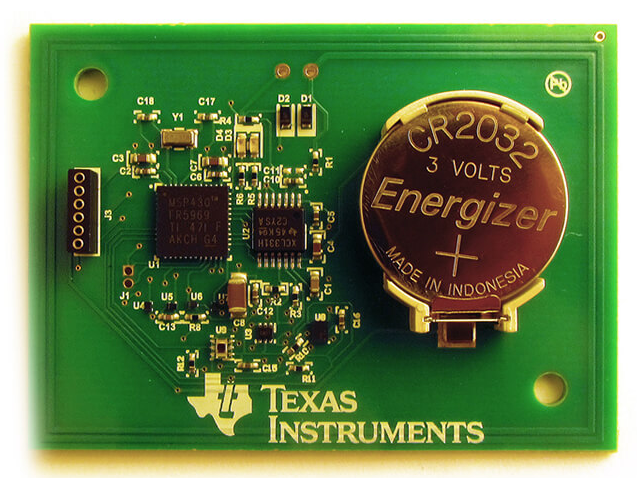
\includegraphics[width=0.3\textwidth]{slike/merilna-naprava-tida.png}
\end{center}
\caption{Merilna naprava TIDA-00524 \cite{dialoger-tida}.}
\label{merilna-naprava-tida}
\end{figure}


\begin{description}
\item[Podatkovni model meritvene naprave TIDA-00524.] Podatkovni model temelji iz podatkov izvoženih iz spletne aplikacija v okviru magistrskega dela Senzorski moduli NFC in varnost podatkov \cite{magistrska-crnigoj}:

\begin{itemize}
\item  zapis datoteke v formatu CSV (.csv),
\item  vrednosti so ločene z znakom vejica (,),
\item  osnovni podatki o meritvi se začnejo z znakom \#,
\item  takoj za osnovnimi podatki so definirana imena vrednosti meritve,
\item  datum je zapisan v obliki leto--dan--mesec (yyyy-MM-dd),
\item  čas je zapisan v obliki ura:minuta:sekunda (HH:mm:ss),
\item  temperatura, relativna vlaga in svetloba so zapisane v decimalnih številih.
\end{itemize}
\end{description}


Merilna naprava RHT10 z USB vmesnikom za enostavno namestitev in prenos podatkov. Beleži senzorske podatke o temperaturi (T) in relativni vlagi (RH). 
Ima možnost več intervalnih vrednosti - od 2 sekundi do 24 ur (slika~\ref{merilna-naprava-rht10}) \cite{rht10-dialogger}.

\begin{figure}[h]
\begin{center}
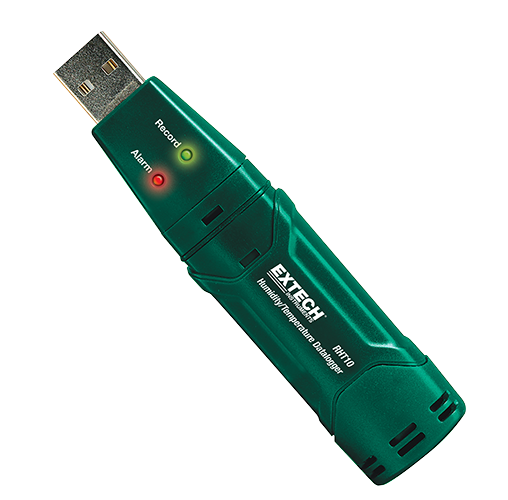
\includegraphics[width=0.3\textwidth]{slike/merilna-naprava-rht10.png}
\end{center}
\caption{Merilna naprava RHT10 \cite{rht10-dialogger}}
\label{merilna-naprava-rht10}
\end{figure}


\begin{description}
\item[Podatkovni model meritvene naprave]\textbf{RHT10:}
\begin{itemize}
\item zapis datoteke v tekstovnem formatu (.txt),
\item vrednosti so ločene z znakom za skok v naslednji odstavek (TAB),
\item osnovni podatki so ločeni z dvema znakoma večje ($>>$),
\item osnovni podatki in imena vrednosti meritve se ločujejo z vrstico, ki je sestavljna iz znakov minus ($-$),
\item datum je zapisan v obliki dan--mesec--leto (dd-MM-yyyy),
\item čas je zapisan v obliki ura:minuta:sekunda (HH:mm:ss),
\item temperatura, relativna vlaga in rosišče so zapisane v decimalnih številih.
\end{itemize}
\end{description}


\noindent Tretji podatkovni model smo za potrebe testiranja definirali kot simulirane meritve hladne verige. Zaradi ročno ustvarjenih podatkov smo ta tip naprave poimenovali kar 'Generated'.


\begin{description}
\item[Glavne lastnosti podatkovnega modela]\textbf{Generated:}
\begin{itemize}
\item podatke se generira direktno v spletni aplikaciji,
\item določi se začetni datum in čas meritve,
\item določi se časovni interval v sekundah,
\item poljubno se dodaja število zapisov z isto temperaturo (°C), \\ relativno vlago (\%) in lokacijo, kjer želimo simulirati meritev.
\end{itemize}
\end{description}

\chapter{Uporabljene tehnologije}
\label{uporabljene-tehnologije}



\section{Podatkovna baza}

Na področju informacijskih sistemov je osnovni vir informacij podatkovna baza, ki vsebuje zbirko shem, tabel, poizvedb, poročil, pogledov in drugih objektov. Upravljamo jo preko sistema za upravljanje baz podatkov. V grobem ločimo relacijske od nerelacijskih. Prve so najbolj razširjene in temeljijo na množici relacij, kjer je vsaka relacija tabela z vrsticami in stolpci. Nerelacijske opredeljuje visoka fleksibilnost, katero dosežejo tako, da nimajo v naprej definirane sheme.
Primeri sistemov za upravljanje relacijskih baz podatkov so MySQL, Oracle, PostgreSQL, nerelacijskih pa MongoDB, Redis, Elasticsearch \cite{podatkovne-baze}.

V diplomski nalogi smo uporabili relacijsko podatkovno bazo s sistemom za upravljanje MySQL \cite{mysql-baza}. Do podatkov smo dostopali preko spletnega vmesnika \verb=phpMyAdmin= \cite{phpmyadmin-framework}.

\section{Spletni strežnik}

Spletni strežnik je sistem, ki obdeluje zahteve preko protokola HTTP.
Njegove osnovne naloge so shranjevanje, obdelava in pošiljanje spletnih strani odjemalcem. Tipični primeri spletnih strežnikov so Apache, Nginx, Microsoft IIS. Vsak iz med njih podpira določene skriptne jezike kot so PHP, ASP, JavaScript \cite{spletni-strezniki}.

V diplomski nalogi smo za razvoj spletne aplikacije izbrali skriptni jezik PHP, ki ima od verzije 5.4.0 vgrajen spletni strežnik za lokalni razvoj, katerega na zahtevo zaženemo preko ukazne vrstice z ukazom \verb=php artisan serve=.

\section{Spletna aplikacija}

Skupek dinamičnih spletnih strani, ki omogočajo izvajanje akcij in opravil katerih spremembe se odražajo nad podatki, imenujemo spletna aplikacija. Glavne lastnosti le-te so neodvisnost od operacijskega sistema, dostopnost, centraliziran nazor in varnost. Zaradi omenjenih lastnosti je potreba po hitrem razvoju spletnih aplikacij vse večja. V ta namen razvijalci uporabljajo ogrodja, ki imajo temeljne gradnike že vnaprej definirane.

Ogrodje Laravel je v zadnjih letih popularno pri razvijalcih v programskem jeziku PHP. Njegov začetek beležimo junija 2011 z prvo verzijo, danes pa je aktualna že šesta, ki sledi zadnjim standardom na področju spletnega razvoja \cite{laravel-main-page}. 

\begin{description}
	
	\item[Nekaj glavnih gradnikov omenjenega]\textbf{ogrodja:}
	
	\begin{itemize}
		\item arhitektura MVC,
		\item vse potrebno za delo z avtentikacijo uporabnika,
		\item konfigurirana obravnava napak in izjem,
		\item odpravljanje najpogostejših tehničnih ranljivosti,
		\item podpora za integracijo predpomnilniških sistemov,
		\item konfiguracija usmerjanja URL-jev,
		\item podpora za integracijo e-poštnih storitev.
		
	\end{itemize}
\end{description}

Za hitrejši razvoj spletnih aplikacij v primerih, ko potrebujemo napredne grafične komponente, razvijalci dodatno izbirajo po predlogah HTML. Predloga HTML običajno vsebuje grafične komponente kot so gumbi, opozorilne kompomente, tipografski elementi, spletni obrazci, grafi in tabele.

Dinamična komunikacija med ogrodjem in grafičnimi komponentami v spletni aplikaciji običajno poteka v obliki spletne storitve REST. Njen namen je definiranje principov, ki opisujejo na kakšen način so viri definirani in naslovljeni, pri katerem se uporabljajo metode protokola HTTP. Te metode so lahko GET, POST, PUT ali DELETE, vsak vir podatkov pa ima svoj URL \cite{protokol-rest}.


\section{Programska oprema}

Pri razvoju spletne aplikacije smo uporabili programsko orodje Intellij IDEA podjetja jetBrains. Produkt je na voljo v plačljivi in zastonjski verziji, namenjen razvijalcem v programskem jeziku Java, med drugim pa nudi podporo tudi za programski jezik PHP. Omogoča tudi integracijo s sistemi za nadzor verzij programske kode, v našem primeru s sistemom Git \cite{intellij-idea}.

Git je sistem za upravljanje z izvorno kodo, s katerim lahko nadzorujemo spremembe, omogoča sodelovanje več razvijalcev na istem projektu, obenem pa nam kadarkoli zagotavlja obnovitev kode na prejšnjo - zgodnejše stanje \cite{sistem-git}.

Za beleženje in vodenje nalog v okviru diplomske naloge smo uporabili spletni servis GitHub. V osnovi omenjeni servis ponuja repozitorije Git v oblaku, omogoča pa tudi distribuirano upravljanje z izvorno kodo, kontrolo dostopa in storitve za razvoj v skupini preko spletnega grafičnega vmesnika \cite{github}.



\chapter{Analiza, načrtovanje in arhitektura}
\label{analiza-nacrtovanje-arhitektura}

V poglavju najprej opredelimo funkcionalne in nefunkcionalne zahteve. V nadaljevanju podrobno opišemo podatkovni model, zaslonske predloge in arhitekturo aplikacije.


\section{Analiza}

Pred izvedbo smo definirali zahteve delovanja spletne aplikacije, ki smo jih razdelili v funkcionalne in nefunkcionalne.


\subsection{Funkcionalne zahteve}

\begin{itemize}
\item Spletna aplikacija naj bo zavarovana in dostopna z uporabniškim imenom in geslom.

\item Vloge uporabnikov so razdeljene na administratorje (ang. Administrator), urednike (ang. Editor) in obiskovalce (ang. User).  

\item Administrator naj ima dostop do vseh funkcionalnosti aplikacije vključno s funkcionalnostmi, ki omogočajo upravljanje z uporabniki (potrditev novega uporabnika in spreminjanje njegove vloge).

\item Urednik naj ima:
	\begin{itemize}
		\item vse funkcionalnosti obiskovalca,
		
		\item možnost uvoza dveh različnih tipov meritev,

		\item možnost generiranja podatkov meritve,

		\item za vsako meritev možnost brisanja, urejanja in izvoza v datoteko PDF,

		\item možnost pregleda, dodajanje in urejanje živil,

		\item možnost pregleda, dodajanja in urejanja lokacij,

		\item možnost pregleda tipov senzorjev.
	\end{itemize}

\item Obiskovalec naj ima:
	\begin{itemize}
		\item celoten seznam, možnost iskanja in filtriranja vseh uvoženih ali generiranih meritev,
		
		\item vidi podroben prikaz in analizo podatkov o meritvi,
		
		\item na podlagi temperature sistem napove preostalo dobo uporabnosti živila.
	\end{itemize}
	
\item Uredniki in obiskovalci se morajo pred prvo uporabo registrirati z naslednjimi podatki: ime in priimek, e-pošta in geslo.

\item Po registraciji mora urednika ali obiskovalca potrditi administrator.

\item Administrator prejme obestilo o novem uporabniku na e-pošto.

\item Potrjeni uporabnik prejme obvestilo na registracijsko e-pošto.

\item Sistem naj prikaže čas trajanja meritve po lokacijah, izračuna največje in najmanjše vrednosti in obvesti o preseženih proporočenih vrednostih v posamezni meritvi.

\item Za potrebe simuliranja meritev in lažjega testiranja aplikacije naj bo dodan generator podatkov.

\end{itemize}


Različne vloge uporabnikov v spletni aplikaciji smo predstavili tudi z diagramom primera uporabe (slika~\ref{diagram-uporabe-userjev}).

\begin{figure}[h]
\begin{center}
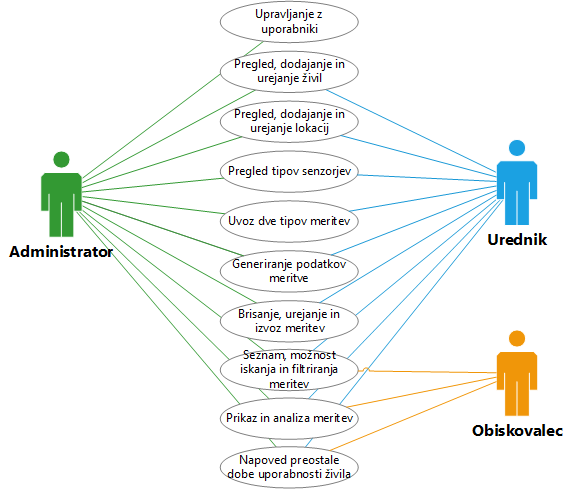
\includegraphics[width=\textwidth]{slike/Use-case-userjev.png}
\end{center}
\caption{Diagram primera uporabe različnih vlog uporabnikov.}
\label{diagram-uporabe-userjev}
\end{figure}


\subsection{Modela za izračun preostale dobe uporabnosti}
\label{modela-za-izracun-sl}

V diplomski nalogi smo za izračun preostale dobe uporabnosti živila za primerjavo uporabili dva različna modela.

\begin{description}

	\item[Model CSIRO] (Commonwealth Scientic and Industrial Research): Razvit je bil v avstralski organizaciji, po kateri je dobil tudi ime. Definiran je s preposto matematično enačbo za razvoj bakterij v živilu \cite{magistrska-marolt}:
	
	\begin{align}
		k = (0,1T + 1)^2				\nonumber \\
       	SL = SL_{ref} - t \times k		\nonumber
	\end{align}
	
	Enačba za izračun preostale dobe uporabnosti po modelu CSIRO na osnovi izmerjene temperature $T$ v časovnem intervalu $t$ določi preostalo dobo uporabnosti $SL$ z upoštevanjem podane referenčne dobe uporabnosti $SL_{ref}$.
	
	\item[Model]\textbf{SAL:} Zasnovan je bil predvsem za morsko hrano. Uporablja tabelo (\ref{tab:tabela-sal}), ki ima za vsako temperaturo navedeno koliko časa je živilo uporabno, če je ves čas hranjeno na tej temperaturi \cite{magistrska-marolt}. 
	
	\begin{align}
		k = t_{ref} / t_{SAL}				\nonumber \\
       	SL = SL_{ref} - t \times k		\nonumber
	\end{align}
	
	Za vrednostjo $t_{SAL}$, ki jo preberemo iz tabele~\ref{tab:tabela-sal}, izračunamo koeficient pokvarljivosti $k$. Preostala doba uporabnosti $SL$ je definirana tako, da od referenčne dobe uporabnosti $SL_{ref}$ odštejemo koeficient v časovnem itervalu $t$.


\begin{table}[h]
\begin{center}
\begin{tabular}{ll|ll|ll|ll}
T(°C) & SL(d) & T(°C) & SL(d) & T(°C) & SL(d) & T(°C) & SL(d) \\ \hline
0     & 8     & 8     & 2,7   & 16    & 1,1   & 24    & 0,75  \\
1     & 6,5   & 9     & 2,35  & 17    & 1     & 25    & 0,73  \\
2     & 5     & 10    & 2     & 18    & 0,92  & 26    & 0,71  \\
3     & 4     & 11    & 1,75  & 19    & 0,89  & 27    & 0,69  \\
4     & 3,5   & 12    & 1,5   & 20    & 0,85  & 28    & 0,67  \\
5     & 3,35  & 13    & 1,4   & 21    & 0,83  & 29    & 0,62  \\
6     & 3,15  & 14    & 1,3   & 22    & 0,8   & 30    & 0,6   \\
7     & 3     & 15    & 1,2   & 23    & 0,78  &       &      
\end{tabular}
\caption{Vrednosti za določitev dobe uporabnosti $SL$ v dnevih pri podani temperaturi hranjenja.}
\label{tab:tabela-sal}
\end{center}
\end{table}
	
\end{description}

\clearpage

\subsection{Nefunkcionalne zahteve}

\noindent \textbf{Varnost}

Zaradi zagotavljanja ustrezne varnosti smo poskrbeli za izvedbo identifikacije, avtentikacije, avtorizacije in beleženja uporabnikov spletne aplikacije (ang. IAAA)~\cite{IAAA-security}.

Identifikacija je v našem primeru e-pošta uporabnika, z ustreznim geslom pa preverimo avtentikacijo oziroma prisotnost uporabnika. Zaradi lažje uporabnosti se nadaljnje preverjanje prisotnosti preverja na podlagi seje, ki ima aktivnost nastavljeno na 2 minute. 

Na nivoju avtorizacije imamo poskrbljeno dva nivoja uporabnikov – urednik in administrator. Privzeto se ob registraciji dodeli vloga neodobrenega urednika, ki še nima dostopa do vsebin, dokler administratorska vloga ne potrdi omenjeno vlogo.

Za zadnji sklop varnosti beležimo še dnevnik prijav uporabnikov. Pri tem nam je v pomoč programsko ogrodje Laravel s knjižnico Monolog~\cite{laravel-monolog}, kjer z enostavnim ukazom shranimo vsako prijavo uporabnika v log datoteko na direktorij strežnika aplikacije. \\

\noindent \textbf{Obravnava napak}

Ena iz med pomembnih nefunkcionalnih zahtev je tudi obravnava napak v sistemu. Obravnavamo strežniške (5xx) in odjemalčeve napake (4xx). 


Na nivoju ogrodja imamo zagotovljeno avtomatsko beleženje napak v log datoteko. V sami predlogi pa imamo poskrbljeno tudi za izpis napake uporabniku.

Primer izvorne kode za izpis napak uporabniku:

\begin{lstlisting}[language=PHP, style=mystyle]
        <div class="alert alert-danger" role="alert">
            @if ($errors->any())
            <ul id="errors">
                @foreach ($errors->all() as $error)
                <li>{{ $error }}</li>
                @endforeach
            </ul>
            @endif
        </div>
\end{lstlisting}

\vspace{5mm}

\noindent \textbf{Prilagodljiva grafična podoba}

Grafični uporabniški vmesnik smo zasnovali tako, da je preprost in pregleden, ter prilagodljiv na vse vrste ekranov. Pri tem smo dali poudarek na vizualizacijske komponente, kot so grafi in tabele. Izbrali smo odprtokodno predlogo HTML {\tt CoolAdmin}~\cite{cooladmin-html-template}, ki je vsebovala že vnaprej definirane grafične komponente.

Grafične komponente so sestavljene iz kode HTML, datoteke CSS, slik in knjižnic JavaScript.
Primer knjižnice JavaScript, ki skrbi za izris interaktivnih grafov v aplikaciji, je {\tt highcharts.js}~\cite{hightchars-js}.




\section{Načrtovanje in arhitektura}

\subsection{Podatkovni model}

Načrtovanje podatkovnega modela nam je olajšalo kasnejše kreiranje objektov. S pomočjo ER diagrama in preslikave relacij v Migrations funkcionalnost ogrodja Laravel~\cite{laravel-migrations}, smo ustvarili tabele v podatkovni bazi MySQL. Na koncu programske rešitve je bil podatkovni model sestavljen iz enajstih tabel. Te so prikazane na sliki~\ref{database-model}.

\begin{figure}[t]
\begin{center}
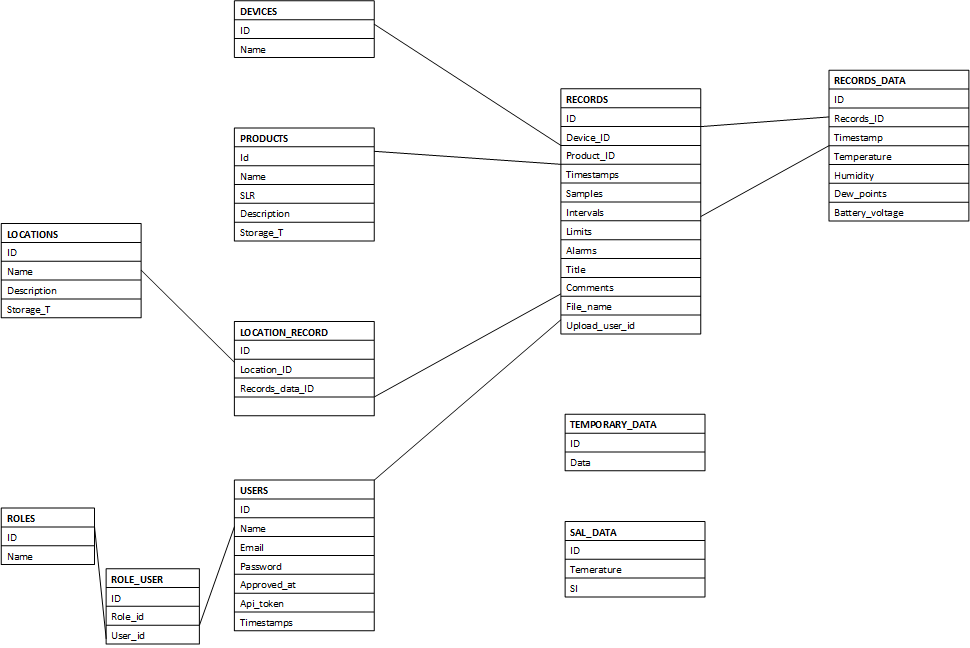
\includegraphics[width=\textwidth]{slike/database_model-updated-for-diploma-1.png}
\end{center}
\caption{ER diagram spletne aplikacije.}
\label{database-model}
\end{figure}

\begin{description}
\item[Tabela USERS] : Predstavlja podatke o uporabniku.
	\begin{itemize}
		\item ID - enolična oznaka uporabnika
		\item Name - ime in priimek uporabnika
		\item Approved\_at - status uporabnika, ki je lahko odobren ali neodobren
		\item Email - email uporabnika
		\item Password - šifrirano geslo uporabnika
		\item API\_token - žeton, ki je uporabljen pri avtentikaciji uporabnika
	\end{itemize}	

\item[Tabela ROLES] : Vsebuje seznam vlog, ki so uporabljene v aplikaciji.
	\begin{itemize}
		\item ID – enolična oznaka vloge
		\item Name – ime vloge (administrator, editor, viewer)
	\end{itemize}

\item[Tabela ROLE\_USER] : Povezovalna tabela med uporabnikom in njegovimi vlogami. 
	\begin{itemize}
		\item ID – enolična oznaka povezave
		\item Role\_ID – enolična oznaka vloge
		\item User\_ID – enolična oznaka uporabnika
	\end{itemize}

\item[Tabela DEVICES] : Vsebuje seznam naprav, ki so vsebovane v meritvi.
	\begin{itemize}
		\item UD – enolična oznaka naprave
		\item Name – ime naprave
	\end{itemize}

\item[Tabela PRODUCTS] : Predstavlja seznam vseh živil, ki so lahko uporabljena v meritvah.
	\begin{itemize}		
		\item ID – enolična oznaka živila
		\item Name – ime živila
		\item SLR – predpisana doba uporabnosti živila
		\item Description – opis živila
		\item Storage\_T – območje priporočene temperature hranjenja živila
	\end{itemize}
	
\item[Tabela LOCATIONS] : Vsebuje seznam vseh lokacij, ki so lahko vsebovane v meritvi.
	\begin{itemize}
		\item ID – enolična oznaka lokacije
		\item Name – ime lokacije
		\item Description – opis lokacije
		\item Storage\_T – območje delovne temperature lokacije
	\end{itemize}
	
\item[Tabela LOCATION\_RECORD] : Povezovalna tabela med lokacijami in meritvami. Ena meritev lahko vsebuje več različnih lokacij.
	\begin{itemize}
		\item ID – enolična oznaka povezave
		\item Location\_ID – enolična oznaka lokacije
		\item Records\_data\_ID – enolična oznaka posameznega zapisa meritve
	\end{itemize}
	
\item[Tabela RECORDS] : Vsebuje seznam vseh uvoženih ali generiranih meritev.
	\begin{itemize}
		\item ID – enolična oznaka meritve
		\item Device\_ID – enolična oznaka naprave
		\item Product\_ID – enolična oznaka živila
		\item Timestamps – avtomatsko generirana časovna polja (created\_at, updated\_at), ki predstavlja čas uvoza in čas zadnje spremembe meritve
		\item Samples – število zapisov v eni meritvi
		\item Intervals – časovni interval med posameznimi zapisi meritve (enota milisekunda)
		\item Limits – polje, ki vsebuje izračunane podatke o robnih številkah meritve
		\item Alarms – polje za opozorila ugotovljena iz meritve
		\item Title – ime posamezne meritve
		\item Comments – komentarji meritve
		\item File\_name – ime uvožene datoteke
		\item Upload\_user\_id – enolični identifikator uporabnika, ki je uvozil meritev
	\end{itemize}
	
\item[Tabela RECORDS\_DATA] : Vsebuje zapis posamezne meritve. Ena meritev ima več posameznih zapisov, medtem ko je lahko zapis vsebovan samo v eni meritvi.
	\begin{itemize}
		\item ID – enolična oznaka zapisa
		\item Records\_ID – enolična oznaka meritve
		\item Timestamp – točen čas zapisa
		\item Temperature – izmerjena temperatura v °C
		\item Humidity – izmerjena relativna vlaga v procentih
		\item Dew\_points – izmerjeno rosišče
		\item Battery\_voltage – napetost baterije merilne naprave
	\end{itemize}
	
\item[Tabela TEMPORARY\_DATA] : Tabela vsebuje trajno shranjene podatke, ki so uporabljeni pri procesu shranjevanja meritve.
	\begin{itemize}
		\item ID – enolični identifikator trajno shranjenih podatkov
		\item Data – podatki iz datoteke meritve
	\end{itemize}

\item[Tabela SAL\_DATA] : Tabela vsebuje podatke, ki so uporabljeni pri izračunu preostale dobe uporabnosti živila po modelu SAL.
	\begin{itemize}
		\item ID – enolični identifikator podatka
		\item Temperature – temperatura hranjenja živila
		\item SL – preostala doba uporabe živila
	\end{itemize}
\end{description}



\subsection{Spletna aplikacija}

Spletna aplikacija je namenjena uporabnikom, ki so odgovorni za kakovost in varnost hitro pokvarljivih živil. Omogoča uvoz, konfiguracijo, pregled, iskanje in filtriranje meritev v procesu hladne verige. V posamezni meritvi se analizira in vizualizira merljive podatke, izračuna največje in najmanjše vrednosti, prikaže skupni čas trajanja meritve po lokacijah, obvesti o preseženih priporočenih vrednostih. Za vse izmerjene temperature v določenem časovnem obdobju aplikacija napove tudi preostalo dobo uporabnosti živila po modelih CSIRO in SAL \cite{magistrska-marolt}.

V fazi načrtovanja smo naredili prototip aplikacije oziroma zaslonske predloge glavnih funkcionalnosti. Vsaka stran vsebuje na levi strani njihov seznam, kjer so povezave do naslednjih strani. 

Aplikacija vsebuje še prikazno sliko vloge in osnovne informacije uporabnika, logotip ter sekundarno navigacijo, ki ponazarja, kje se nahajamo na strani. Omenjene funkcionalnosti so bile izpuščene iz prototipa, saj niso igrale pomembne vloge.

\begin{figure}[h]
\begin{center}
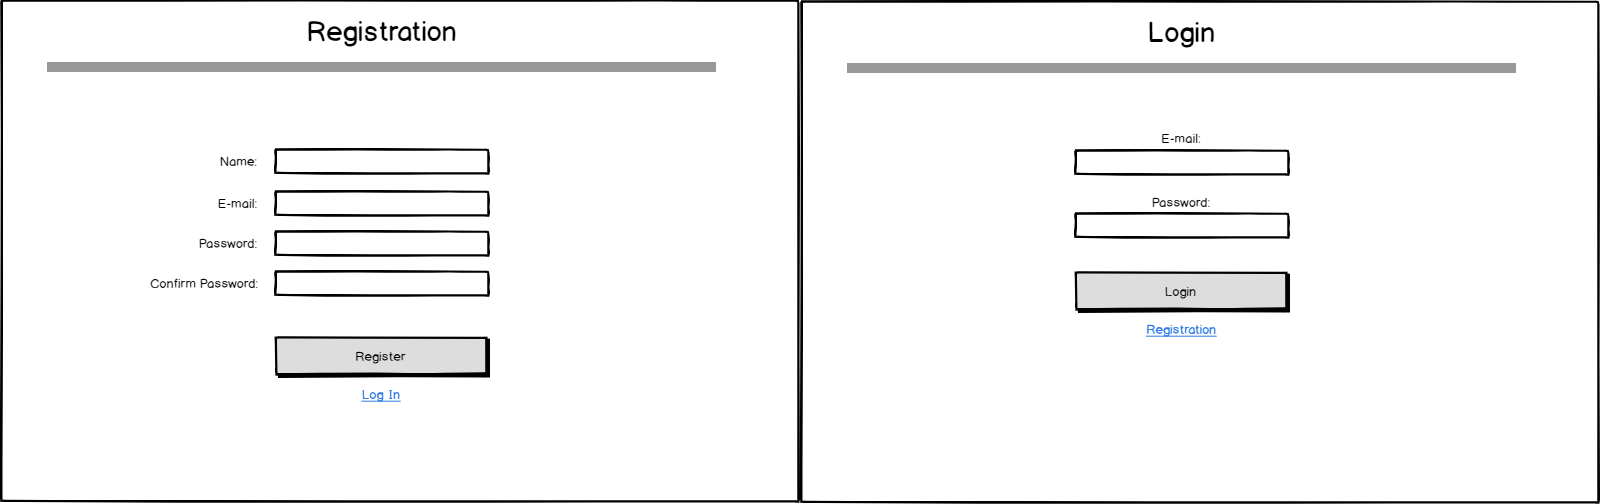
\includegraphics[width=\textwidth]{slike/registration_and_Login-wireframe.png}
\end{center}
\caption{Zaslonska predloga registracije (levo) in prijave (desno).}
\label{registration-login-wireframe}
\end{figure}

Na vstopni strani se prikaže obrazec za prijavo, kot prikazuje slika~\ref{registration-login-wireframe}. Uporabnik mora ob prvem obisku navigirati na stran z registracijo s klikom na povezavo \sn{Registration}.

Neregistrirani uporabnik vnese podatke o imenu, e-pošti naslov in ponovitvi gesla ter klikne na gumb \sn{Register}.

V primeru, da je uporabnik že registriran, na prijavni strani vnesene e-poštni naslov in geslo, klikne na gumb \sn{Login} in v primeru uspešne prijave ga aplikacija preusmeri na seznam meritev.


V primeru uspešne registracije je uporabnik preusmerjen na opozorilno stran, kjer mu sporočimo, da je v postopku potrjevanja (slika~\ref{approval-wireframe}).
Ob izvedeni administratorski potrditvi uporabnik prejme obvestilo na registracijski e-poštni naslov.

\begin{figure}[h]
\begin{center}
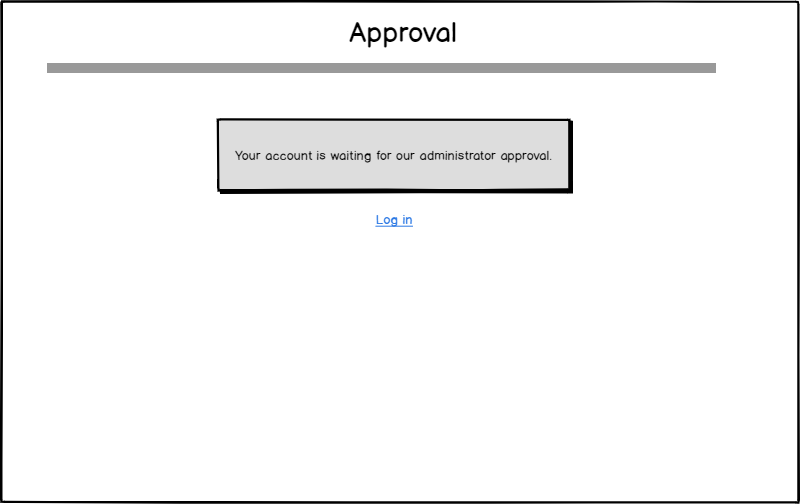
\includegraphics[width=0.5\textwidth]{slike/NotAlloved.png}
\end{center}
\caption{Opozorilna stran o administratorskem potrjevanju.}
\label{approval-wireframe}
\end{figure}


\begin{figure}[h]
\begin{center}
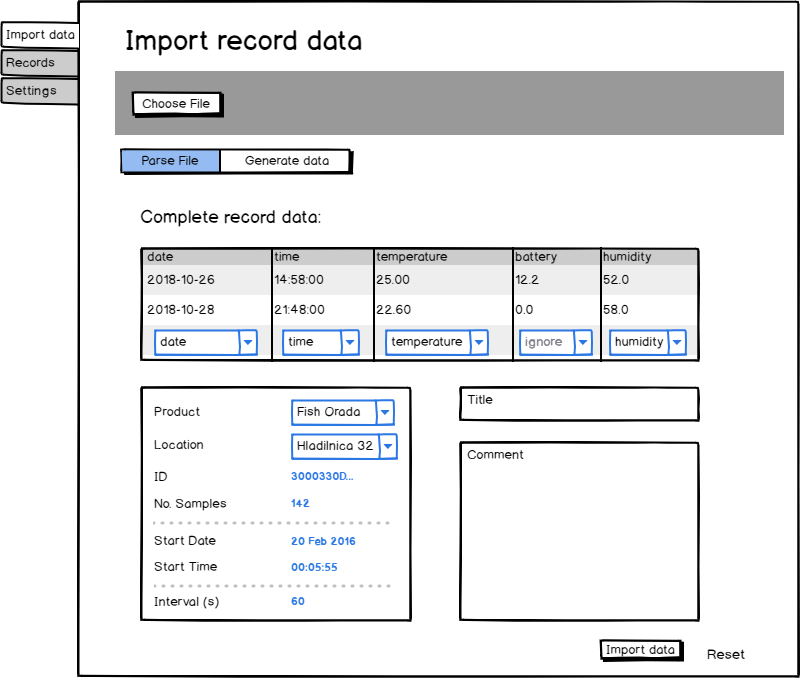
\includegraphics[width=0.5\textwidth]{slike/Import-data.png}
\end{center}
\caption{Spletno okno za uvoz meritev. Na izbiro imamo uvoz datoteke ali generiranje podatkov.}
\label{import-data-wireframe}
\end{figure}

V prvem koraku z gumbom \sn{Choose File} izberemo željeno datoteko v ustreznem formatu. Dovoljena formata omogočata uvoz meritev v tekstovni datoteki ali datoteki CSV (vrednosti ločene z vejico). Takoj po izbiri sistem preveri datoteko in prikaže nadaljnje korake (slika~\ref{import-data-wireframe}).

Sledi konfiguracija vhodnih podatkov, kjer aplikacija prikaže imena vseh stolpcev s primerom dveh vrstic podatkov, vsebovanih v datoteki. Predstavljene stolpce lahko poljubno spreminjamo s stolpci določenih v aplikaciji. Vrednosti, ki jih lahko izbiramo iz spustnega seznama so: datum, čas, temperatura, relativna vlaga, napetost baterije, rosišče ali \sn{--ignore--}. Z zadnjo vrednostjo povemo aplikaciji, da izbrani stolpec pri uvozu meritve izpusti.

\noindent V zadnjem koraku izpolnimo še preostale podatke o meritvi, kot so: 
\begin{itemize}
	\item izbira živila, ki je bilo povezano z meritvami hladne verige. Iz izpustnega seznama \sn{Product} lahko izbiramo živila, ki smo jih predhodno vnesli v aplikaciji. Predstavili smo: izbiro z Ribe – tuna, Ribe – brancin, Svinina, Govedina - mleto meso, Govedina, Piščanec – file,
	
	\item izbira lokacije, kjer je bila opravljena meritev. Iz izpustnega seznama \sn{Location} lahko izbiramo lokacije, ki smo jih predhodno vnesli v aplikaciji,
	
	\item ime meritve v vnosnem polju \sn{Title},
	
	\item komentar meritve v vnosnem polju \sn{Comment}.
\end{itemize}

Informativno se izpišejo tudi podatki o številu zapisov (\sn{No. Samples}), začetku in koncu meritve (\sn{Start Date}, \sn{End Date}) in intervalni vrednosti med zapisi v sekundah (\sn{Interval(s)}). 

S klikom na gumb \sn{Reset} se lahko ponovno nastavi uvožene podatke.

Čisto na koncu s klikom na \sn{Import data} shranimo uvožene podatke v bazo. Po uspešni shranitvi se nam prikaže obvestilo s povezavo do ogleda meritve. V primeru, da pri shranjevanju pride do napake, se uporabniku izpiše opozorilo z opisom težave v rdeči barvi.

\begin{figure}[h]
\begin{center}
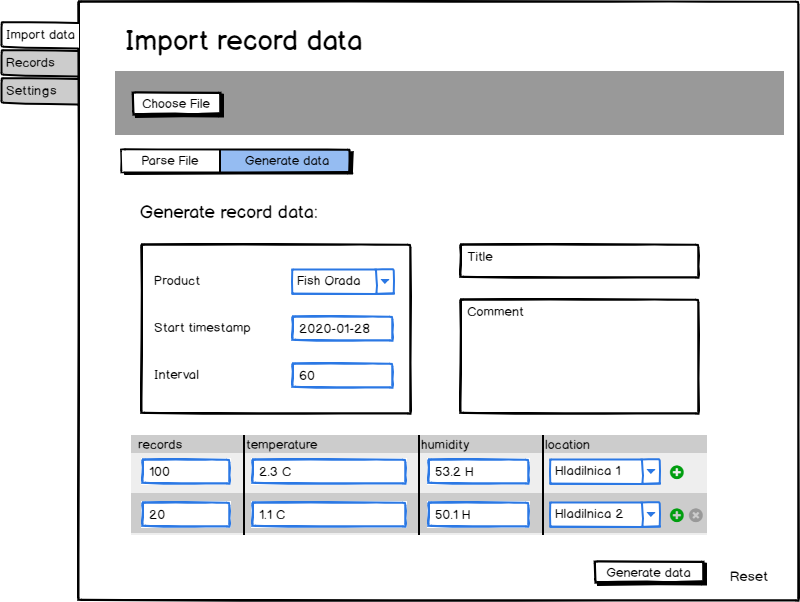
\includegraphics[width=0.5\textwidth]{slike/Import-data-Generate.png}
\end{center}
\caption{Zavihek \sn{Generate data} za ročno generiranje meritev.}
\label{generate-data-wireframe}
\end{figure}

Pri kliku na zavihek \sn{Generate data} se prikaže spletno okno iz slike~\ref{generate-data-wireframe}. Omogoča ročno generiranje meritev, tako da na začetku vnesemo ime in komentar meritve, iz izpustnega seznama izberemo živilo (\sn{Product}) in nastavimo začetni čas (\sn{Start timestamp}) in interval med zapisi v sekundah (\sn{Interval}).

Na naslednjem razdelku vnesemo število in vrednosti posameznih zapisov. V polju \sn{Records} vnesemo število zapisov, v polju \sn{Temperature} temperaturo v ºC, v polju \sn{Humidity} relativno vlago v \% in iz izpustnega seznama \sn{Location} lokacijo.

S klikom na zeleno ikono \sn{plus} poljubno dodajamo nove intervalne vrednosti zapisov. 
S klikom na sivo ikono \sn{X} pa poljubno odstranjujemo intervalne vrednosti zapisov.

Po vnosu podatkov zaključimo s klikom na gumb \sn{Generate data} ali \sn{Reset}. V prvem primeru se po uspešno generirani meritvi prikaže obvestilo s povezavo do ogleda meritve, v drugem pa se vsi podatki brišejo.



\begin{figure}[h]
\begin{center}
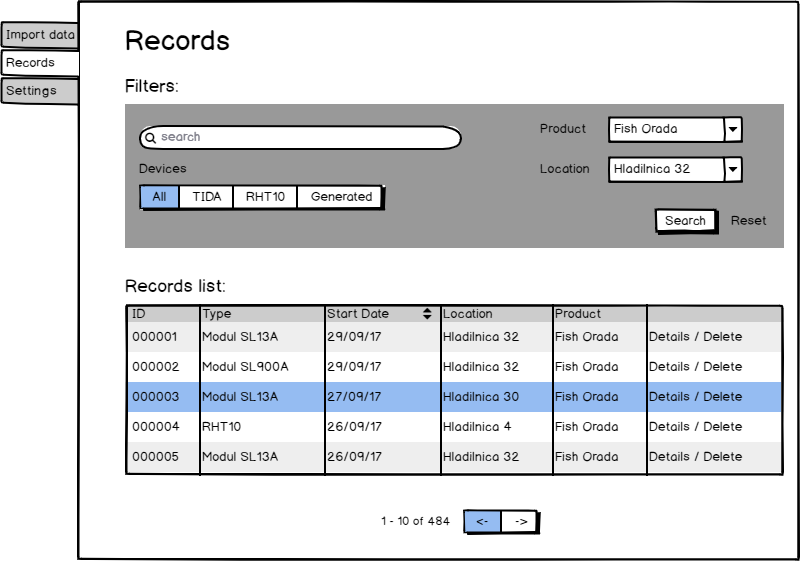
\includegraphics[width=0.5\textwidth]{slike/Records.png}
\end{center}
\caption{Spletno okno za prikaz seznama meritev.}
\label{records-wireframe}
\end{figure}

Na spletnem oknu za prikaz seznama meritev (slika~\ref{records-wireframe}) iz razdelka \sn{Filters} lahko iščemo meritve po različnih kriterijih. Te so:
\begin{itemize}
	\item polje \sn{search} po ključni besedi,
	\item gumbi \sn{All}, \sn{TIDA}, \sn{RHT10}, \sn{Generated} po tipu naprave,
	\item spustni seznam \sn{Product} po imenu živila,
	\item spustni seznam \sn{Location} po imenu lokacije.  
\end{itemize}

S klikom na gumb \sn{Reset} pobrišemo trenutne iskalne kriterije.


Pod razdelkom s filtri se v tabelaričnem seznamu prikazujejo filtrirane meritve z nekaj osnovnimi informacijami in možnostjo ogleda podrobnosti (gumb \sn{Details}) ali brisanjem (gumb \sn{Delete}).

Gumb \sn{Details} omogoča prehod na stran s podrobno analizo meritve.

Na eni strani je prikazano deset meritev. Ostale si lahko ogledamo s klikom na ikoni puščice naprej ali nazaj.

\clearpage

\begin{figure}[h]
\begin{center}
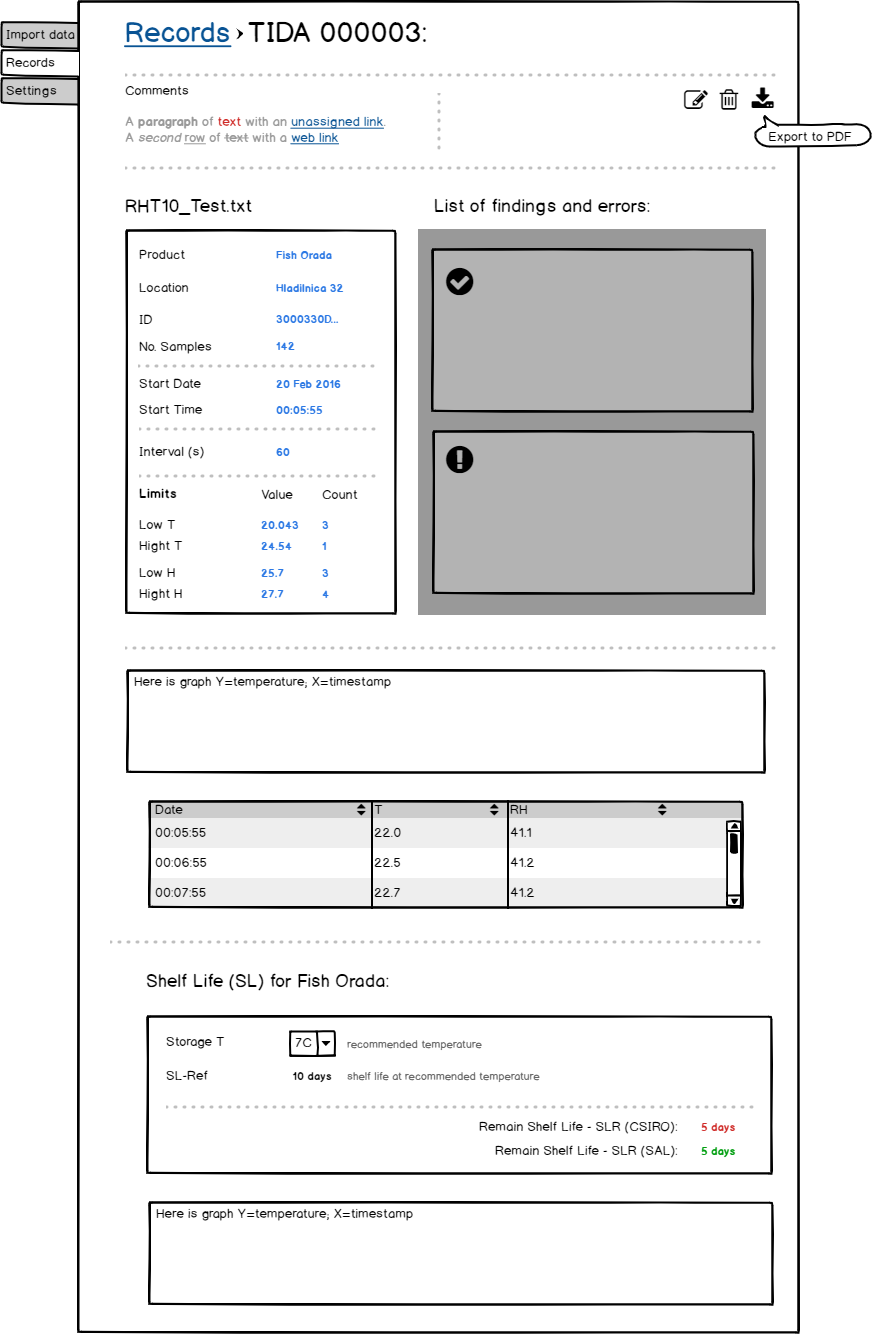
\includegraphics[width=0.5\textwidth]{slike/Record-view.png}
\end{center}
\caption{Zaslonski predlog z podrobnimi informacijami in analizo meritve.}
\label{record-wireframe}
\end{figure}

Na sliki~\ref{record-wireframe} je prikazano, da imamo v skrajnem desnem robu s kliki na ikone možnost urejanja, brisanja ali izvoza meritve v dokument PDF.
Poleg že omenjenih osnovnih informacij meritve se nam v razdelku ugotovitve in opozorila (\sn{Findings and Alerts}) izpišejo morebitna opozorila, celoten čas izven priporočenih temperatur in skupni čas po lokacijah.

Vse meritve se poleg tabelaričnega izpisa prikažejo tudi v grafični obliki.
Graf po Y osi prikazuje temperaturo (levo) in relativno vlago (desno), po X osi pa celotni čas meritve. Črti na grafu določata temperaturo (modra črta) in relativno vlago (črna črta) v odvisnosti od časa.

Ob kliku na ikono znotraj grafa v skrajnem desnem robu imamo možnost pogleda čez celoten ekran, izvoz v različne formate ali tiskanje grafa.

V zadnjem razdelku sta vizualizirana dva modela napovedi preostale dobe uporabnosti živila. Podatek \sn{Storage\_T} prikaže priporočeno temperaturo hranjenja živila, ki je del naše meritve. Podatek \sn{SL-Ref} se nanaša na referenčno dobo uporabnosti živila pri priporočeni temperaturi v število dneh. 

Na desni strani sta z dvema različnima barvama prikazana izračuna za preostalo dobo uporabnosti po modelu CSIRO in SAL.

Graf pri dobi uporabnosti je podoben prvemu, le da vsebuje še dve linearni črti, ki ponazarjata kako se je doba uporabnosti spreminjala skozi čas meritve.

\vspace{5mm}

\begin{figure}[h]
\begin{center}
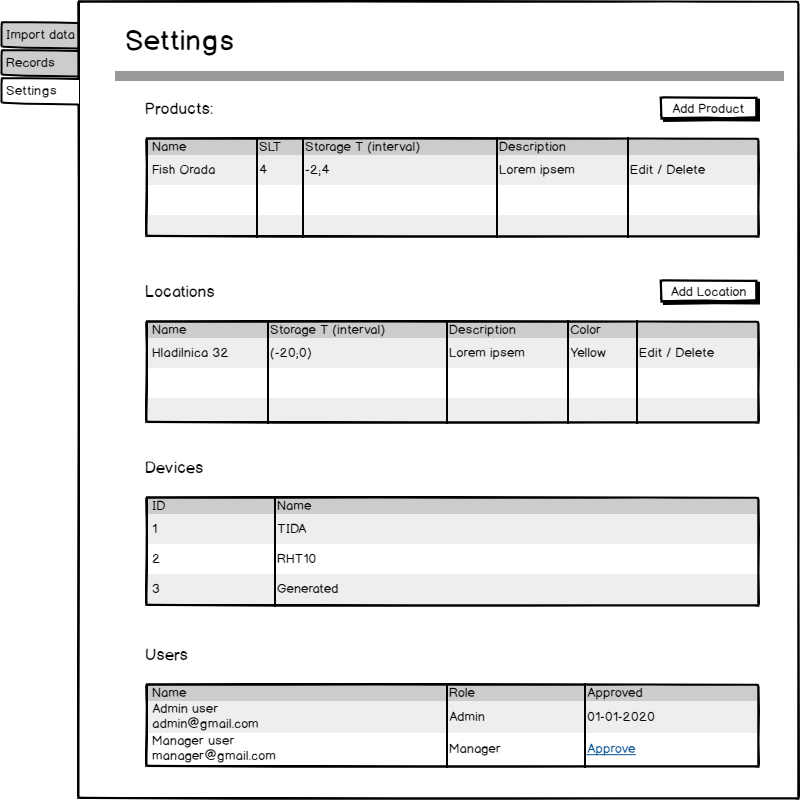
\includegraphics[width=0.5\textwidth]{slike/Settings.png}
\end{center}
\caption{Spletno okno predstavlja stran z nastavitvami.}
\label{settings-wireframe}
\end{figure}

Na spletni strani z nastavitvami so seznami živil, lokacij, naprav in uporabnikov (slika~\ref{settings-wireframe}). Dostop do omenjene strani imajo administratorji in uredniki. 

Seznam živil je predstavljen v razdelku \sn{Products} v obliki tabele. Vsako živilo lahko urejamo ali brišemo. Imamo tudi možnost dodajanja novega živila. 

Seznam lokacij je predstavljen v razdelku \sn{Locations} v oblike tabele. Vsako lokacijo lahko urejamo ali brišemo. Imamo tudi možnost dodajanja nove lokacije.

Seznam naprav je predstavljen v razdelku \sn{Devices}. Seznam naprav lahko samo pregledujemo, saj so že pred-nastavljene v spletni aplikaciji.

Seznam uporabnikov je predstavljen v razdelku \sn{Users}. 
Administrator ima pri neodobrenih uporabnikih možnost odobritve s klikom na gumb \sn{Approve}, ostali uporabniki ne vidijo tega stolpca. 



\subsection{Arhitektura}

Spletna stran je narejena z odprtokodnim ogrodjem Laravel \cite{laravel-main-page}, ki temelji na programskem jeziku PHP \cite{php-jezik}. Ogrodje je arhitekturno zasnovano po vzorcu MVC. 

Princip arhitekturnega vzorca MVC temelji na delitvi aplikacije na tri medsebojno povezane komponente. Model (ang. model) ima odgovornost za podatke, kontroler (ang. controller) vsebuje poslovno logiko in pogled (ang. view) skrbi za prikaz podatkov uporabniku \cite{poglavje_laravel_mvc}.

Slika~\ref{mvc-laravel} prikazuje tok MVC v ogrodju Laravel. Prične se z uporabniškim zahtevkom (ang. request), ki potuje preko usmerjevalnika oziroma naslova URL (ang. route) do kontrolerja. Kontroler običajno pridobi podatke iz podatkovne baze preko modela. Vsa komunikacija od kontrolerja potuje tudi v obratni smeri do pogleda, kjer se uporabniku prikažejo podatki. 

\begin{figure}[h]
\begin{center}
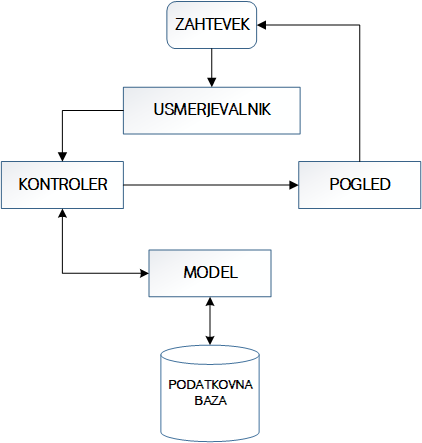
\includegraphics[width=0.4\textwidth]{slike/Laravel-MVC.png}
\end{center}
\caption{Tok MVC v ogrodju Laravel.}
\label{mvc-laravel}
\end{figure}

\clearpage

Dinamični deli aplikacije delujejo po principu spletne storitve REST. Za upravljanje in prikaz dinamičnih delov uporabniku so nam v pomoč različne knjižnice JavaScript kot na primer bootstrap-table.js \cite{bootstraptable} za prikaz podatkov v tabeli in hightcharts.js \cite{hightchars-js} za prikaz podatkov v grafu.






\chapter{Razvoj}
\label{razvoj}

Poglavje podrobno opisuje glavne funkcionalnosti spletne aplikacije. V začetku opišemo način implementacije podatkovne baze in zasnove spletne aplikacije ter storitve, v nadaljevanju pa opišemo posamezne funkcionalnosti z zaslonskimi slikami in pomembnimi odseki izvorne kode.


\section{Podatkovna baza}

Za vir podatkov naše spletne aplikacije smo izbrali podatkovno bazo MySQL in v njej kreirali shemo. Znotraj sheme smo definirali tabele na podlagi modelov, ki so bili narejeni po vzoru ER diagrama iz prejšnjega poglavja.
 
Za implementacijo tabel smo si pomagali s tehnologijo Migrations znotraj ogrodja Laravel. Migrations je zapis definicije tabele v obliki datoteke PHP, ki nam omogoča lažje verzijoniranje, spreminjanje in deljenje med razvojnimi okolji \cite{laravel-migrations}.

\clearpage

Primer programske kode za kreiranje tabele uporabnik s pomočjo tehnologije Migrations Laravel:

\begin{lstlisting}[language=PHP, style=mystyle]
class CreateUsersTable extends Migration {
    public function up() {
        if (!Schema::hasTable('users')) {
            Schema::create('users', function (Blueprint $table) {
                $table->bigIncrements('id');
                $table->string('name');
                $table->string('email')->unique();
                $table->timestamp('email_verified_at')->nullable();
                $table->string('password');
                $table->timestamp('approved_at')->nullable();
                $table->rememberToken();
                $table->timestamps();
            });
        }
    }
}
\end{lstlisting}

Ogrodje Laravel nam omogoča tudi vmesnik ukazne vrstice imenovane Artisan, ki nam olajša razvojno delo z številnimi uporabnimi ukazi, kot so ustvari kontroler (\verb=php artisan make:controller=), počisti predpomnilnik (\verb=php artisan cache:clear=), pokaži listo povezav (\verb=php artisan route:list=) \cite{laravel-artisan}.

Tako smo tudi samo kreacijo tabel izvedli z vmesnikom Artisan ukazne vrstice \verb=php artisan migrate=.

\newpage

\section{Spletna aplikacija in storitev}

Vsaka komponenta MVC spletne aplikacije vsebuje usmerjevalnik, ki sprejme uporabnikove zahtevke HTTP in jih posreduje ustreznemu kontrolerju.
V tabeli~\ref{tabela-url} je seznam in opis vseh usmerjevalnikov aplikacije.

\begin{table}[htbp]
	\centering
	\scriptsize
	{\def\arraystretch{1.4}
	 \begin{tabularx}{\textwidth}{b|zs}
	
	\textbf{naslov URL} & \textbf{metoda HTTP} & \textbf{opis} \\ \hline

/LOGIN & GET & Prijava v aplikacijo. \\
/LOGOUT & GET & Odjava iz aplikacije. \\
/REGISTER & GET & Registracija v aplikacijo. \\
/APPROVAL & GET & Opozorilna stran pred odobritvijo. \\
/IMPORT & GET & Prikaz strani z uvozom meritve. \\
/IMPORT/PARSE & POST & Preverba in razčlenitev meritve. \\
/IMPORT/SAVE & POST & Shranitev meritve. \\
/IMPORT/GENERATE & POST & Shranitev generirane meritve. \\  
/RECORDS & GET & Seznam meritev. \\
/RECORD/$\mathrm{\{}$ID$\mathrm{\}}$ & GET & Ogled posamezne meritve. \\  
/RECORD/EDIT/$\mathrm{\{}$ID$\mathrm{\}}$ & POST & Shranitev sprememb meritve. \\
/RECORD/DELETE/$\mathrm{\{}$ID$\mathrm{\}}$ & DELETE & Izbris meritve. \\
/SETTINGS & GET & Naslov za ogled živil, lokacij, naprav in uporabnikov. \\
/SETTINGS/APPROVE/$\mathrm{\{}$USER\_ID$\mathrm{\}}$ & GET & Naslov za odobritev novega uporabnika. \\ 
/PRODUCT/STORE & POST & Shranitev novega \v{z}ivila. \\ 
/PRODUCT/EDIT/$\mathrm{\{}$ID$\mathrm{\}}$ & POST & Shranitev sprememb živila. \\
/PRODUCT/DELETE/$\mathrm{\{}$ID$\mathrm{\}}$ & DELETE & Izbris živila. \\
/LOCATION/STORE & POST & Shranitev nove lokacije. \\
/LOCATION/EDIT/$\mathrm{\{}$ID$\mathrm{\}}$ & POST & Shranitev sprememb lokacije. \\
/LOCATION/DELETE/$\mathrm{\{}$ID$\mathrm{\}}$ & DELETE & Izbris lokacije. \\

	\end{tabularx}
	}
	\caption{Seznam in opis vseh usmerjevalnikov aplikacije.}
	\label{tabela-url}
\end{table}


\section{Prijava, odjava, registracija in potrditev uporabnika}

Funkcionalnosti povezane z avtentikacijo in avtorizacijo smo povezali v eno smiselno komponento MVC, ki vsebuje dva modela; uporabnik (ang. User) in pravilo (ang. Role), tri kotrolerje in poglede; prijava (\verb=LoginController=, \verb=login.blade.php=), registracija (\verb=RegisterController=, \verb=register.blade.php=) in potrditev (\verb=ApprovalController=, \verb=approval.blade.php=).

\begin{figure}[h]
\begin{center}
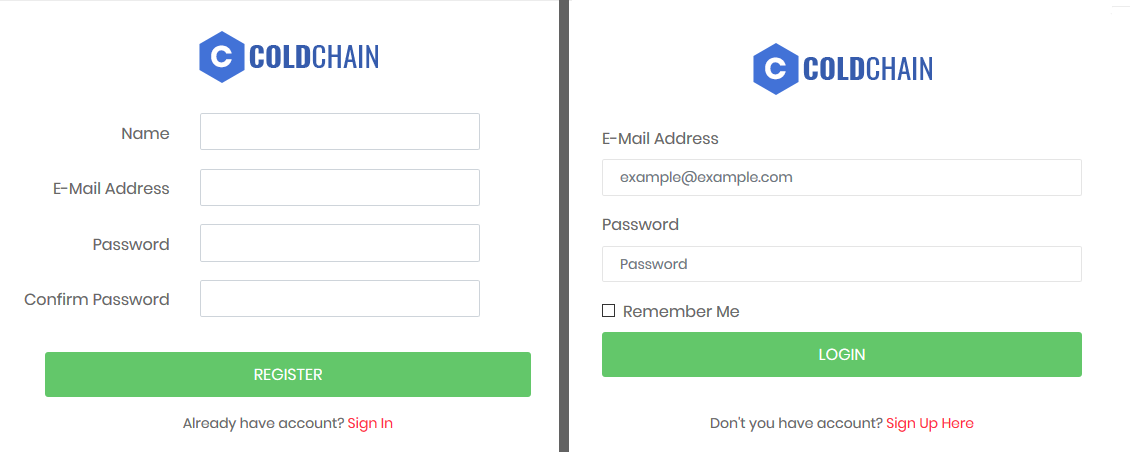
\includegraphics[width=\textwidth]{slike/registration_login.png}
\end{center}
\caption{Zaslonska posnetka registracije (levo) in prijave (desno).}
\label{ss-registration-login}
\end{figure}

Uporabniki se morajo pred uporabo aplikacije najprej prijaviti ali registrirati (slika~\ref{ss-registration-login}). Novo registrirani uporabnik privzeto dobi vlogo obiskovalca. Le-tega pa mora administrator, pred nadaljnjo uporabo, odobriti.

Primer glavne funkcije potrditvenega kontrolerja:

\begin{lstlisting}[language=PHP, style=mystyle]
public function handle($request, Closure $next)
{
    if (!auth()->user()->approved_at) {
        return redirect()->route('approval');
    }
    return $next($request);
}
\end{lstlisting}

\newpage 

Primer izvorne kode pogleda pri neodobrenem uporabniku:

\begin{lstlisting}[language=PHP, style=mystyle]
@extends('layouts.login')
@section('content')
<div class="container">
    <div class="login-logo">
        <a href="{{ route('login') }}">
            <img src="{{ asset('images/icon/logo-blue.png') }}" alt="{{ config('app.name') }}">
        </a>
    </div>
    <div class="login-form text-center">
        <p>Your account is waiting for our administrator approval.</p>
        <p>Please check later.</p>
        <p><a href="{{ route('login') }}" class="btn btn-link">Sign in</a></p>
    </div>
</div>
@endsection
\end{lstlisting}

Rezultat pogleda, kot ga vidi uporabnik, je prikazan na sliki~\ref{ss-approval}.

\begin{figure}[h]
\begin{center}

\includegraphics[width=0.7\textwidth]{slike/approval.png}
\end{center}
\caption{Zaslonski posnetek pogleda pri neodobrenem uporabniku.}
\label{ss-approval}
\end{figure}

\newpage

\begin{figure}[h]
\begin{center}
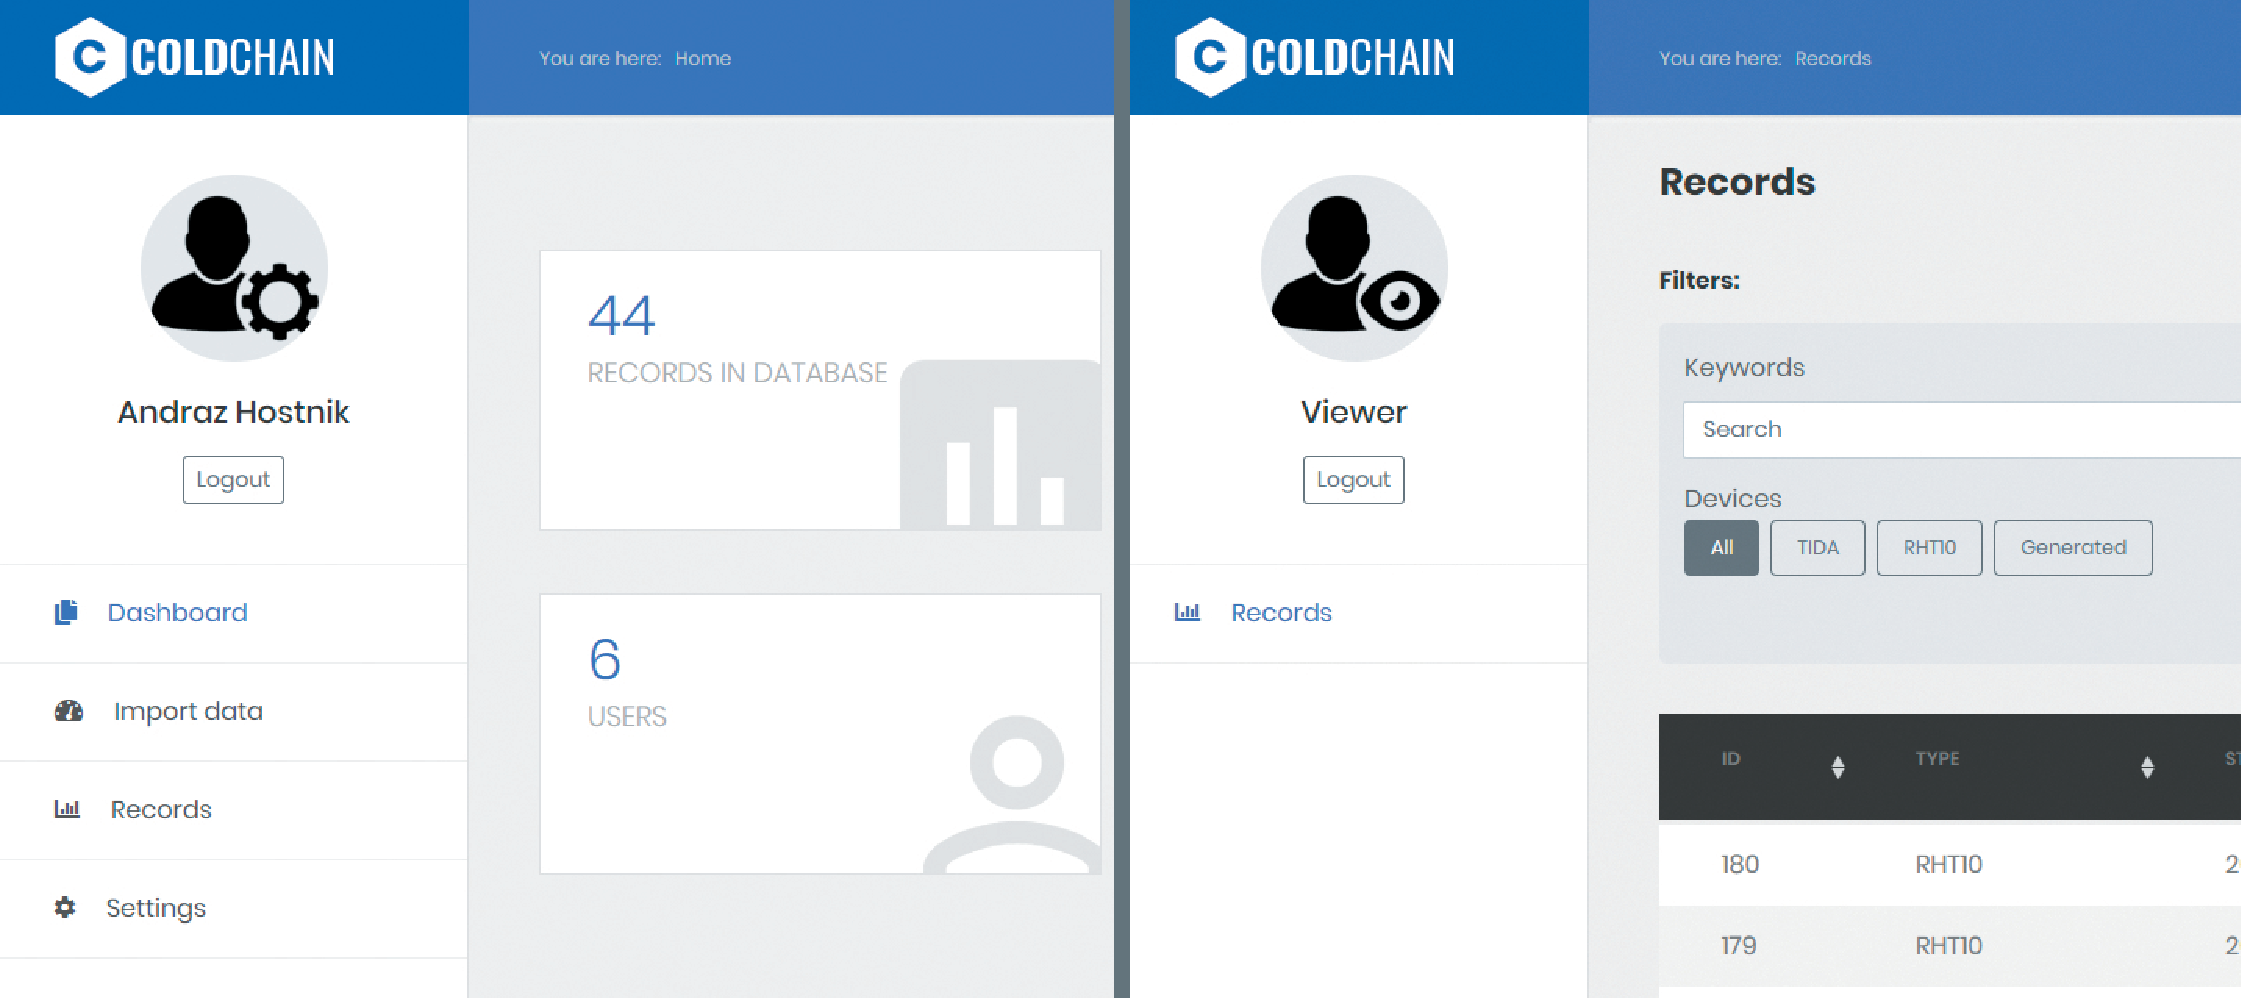
\includegraphics[width=\textwidth]{slike/logout-obiskovalec.pdf}
\end{center}
\caption{Zaslonski posnetek prve avtorizirane strani za administratorje in urednike (levo) ter obiskovalce (desno).}
\label{ss-obiskovalec}
\end{figure}

Po prijavi odobrenega uporabnika se odpre prva avtorizirana stran, ki tako kot vse preostale, vsebuje navigacijsko vrstico, logotip, prikazno sliko, ki ponazarja vlogo uporabnika, in povezavo do odjave. (slika~\ref{ss-obiskovalec} levo).

Uporabniki z vlogo obiskovalec vidijo drugačno navigacijsko vrstico, kot ostali uporabniki, saj imajo dostop omogočen samo do strni z meritvami (slika~\ref{ss-obiskovalec} desno). 



\section{Uvoz in generiranje meritev}
\label{uvoz-in-generiranje-meritev}

Ena iz med glavnih funkcionalnosti urednika je uvoz ali generiranje meritev. 
Za uvoz meritve smo razvili posebno logiko prepoznave podatkov o meritvah v uvoženi datoteki. Na podlagi determinatorja, števila in imena stolpcev v fazi shranjevanja ponudimo uporabniku možnost konfiguracije meritvenih podatkov.

\clearpage

Primer privatne funkcije znotraj kontrolerja \verb=ImportController= za prepoznavo meritev tipa TIDA:

\begin{lstlisting}[language=PHP, style=mystyle]
// P A R S E   T I D A   files
// input - data of file
// output - object record
private function parseTIDAFiles($data){
    $record = new Records();
    $record->device_id = 'TIDA';
    // check if string ;; exist and remove this
    $lastEl = key(array_slice($data[0], -1, 1, true));
    if(array_key_exists(0, $data) && strpos($data[0][$lastEl], ';;') !== false){
        $data = $this->removeWhiteString($data);
    }
    // parse headers data
    foreach($data as $key => $row){
        if(array_key_exists(1, $row)){
            if($row[1] == 'Title') $record->title = $row[2];
            if($row[1] == 'Description') $record->comments = $row[2];
            if($row[1] == 'Location') $record->location_id = $row[2];
            if($row[1] == 'StartDate') $record->start_date = $row[2] . ' ' . $row[3];
            if($row[1] == 'EndDate') $record->end_date = $row[2] . ' ' . $row[3];
            if($row[1] == 'LogInterval(s)') $record->intervals = $row[2];
            if($row[1] == 'Measurements') $record->samples = $row[2];
        }
        if($row[0]  != '#' ){ 
            $record->nr_header_rows = $key; 
            break;
        }
    }
    return $record;
\end{lstlisting}


Na sliki~\ref{ss-import-data} smo v razdelku \sn{Define headers data} pri stolpcu \sn{light} iz izpustnega seznama izbrali \sn{--ignore--}, kar pomeni ignoriranje omenjene vrednosti pri uvozu v bazo. V spodnjem desnem delu je med drugim razvidno tudi, da gre za tip naprave TIDA, sami pa smo izbrali, da gre za produkt Ribe - tuna na lokaciji Hladilnik 1. S klikom na modri gumb \sn{Import Data} se meritev shrani.


\begin{figure}[h]
\begin{center}
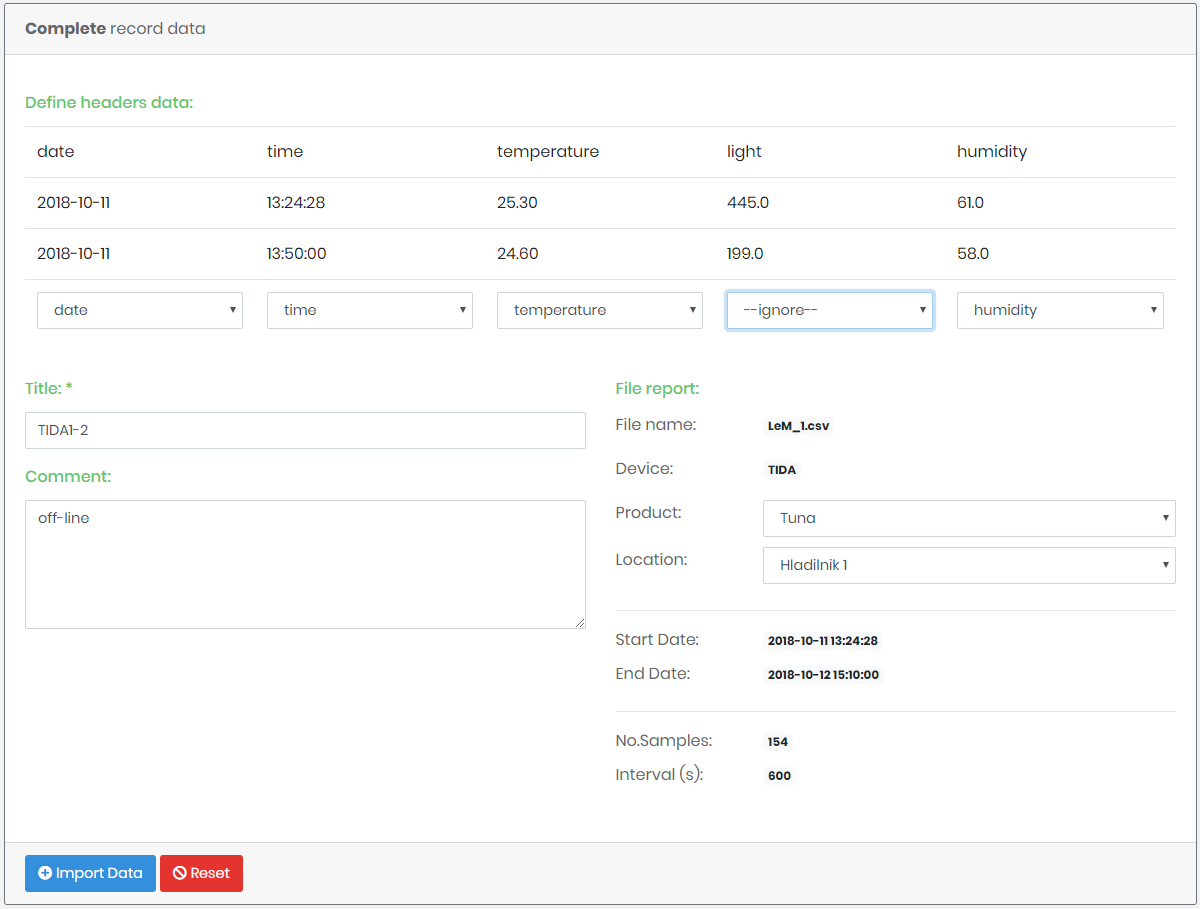
\includegraphics[width=\textwidth]{slike/import_data_tida.png}
\end{center}
\caption{Zaslonski posnetek shranjevanja meritve z imenom \sn{TIDA1-2}.}
\label{ss-import-data}
\end{figure}


\begin{figure}[h]
\begin{center}
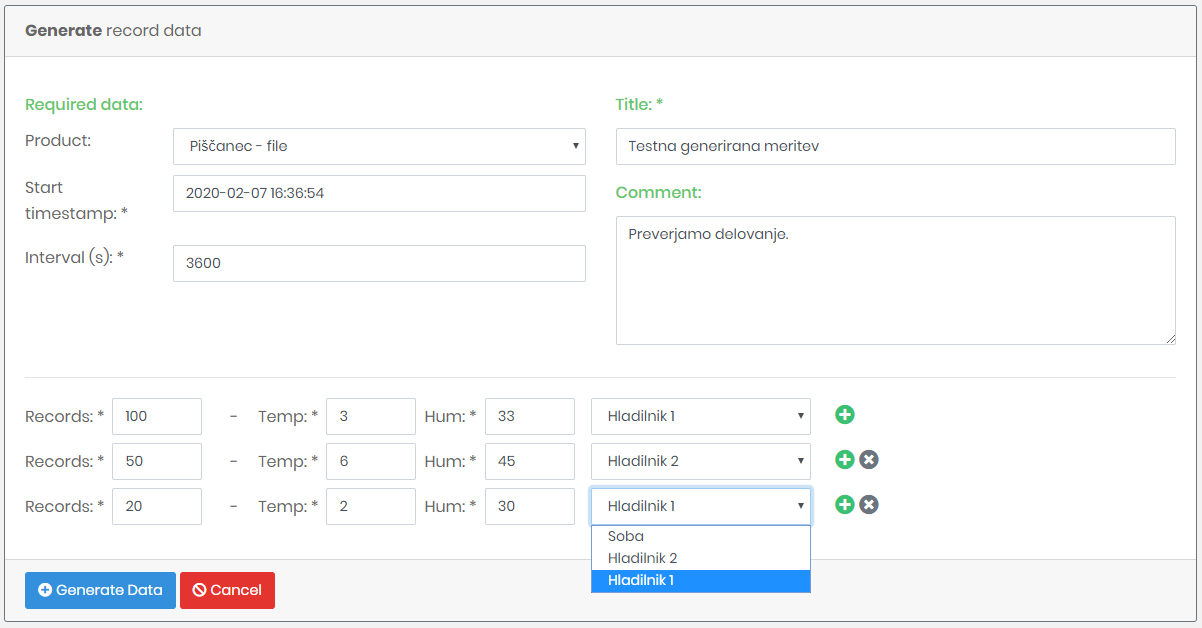
\includegraphics[width=\textwidth]{slike/generate_data.png}
\end{center}
\caption{Slika prikazuje primer generiranja meritve.}
\label{ss-generate-data}
\end{figure}

Slika~\ref{ss-generate-data} prikazuje primer generiranja meritve pri kateri smo pod razdelkom \sn{Required data} izbrali produkt Piščanec – file, začetek meritve ob 16:36:54 dne 7.2.2020 z intervalom 3600 sekund, kar bo predstavljajo podatek o meritvi z intervalom ene ure. V nadaljevanju smo določili tri generirane sklope. Prvi vsebuje 100 zapisov z temperaturo 3 °C, vlažnostjo 33 \% na lokaciji Hladilnik 1, drugi 50 zapisov z temperaturo 6 °C, vlažnostjo 45 \% na lokaciji Hladilnik 2 in tretji 20 zapisov z temperaturo 2 °C, vlažnostjo 30 \% na lokaciji Hladilnik 1. S klikom na modri gumb \sn{Generate Data} se meritev shrani (slika~\ref{ss-import-success}).


\begin{figure}[h]
\begin{center}
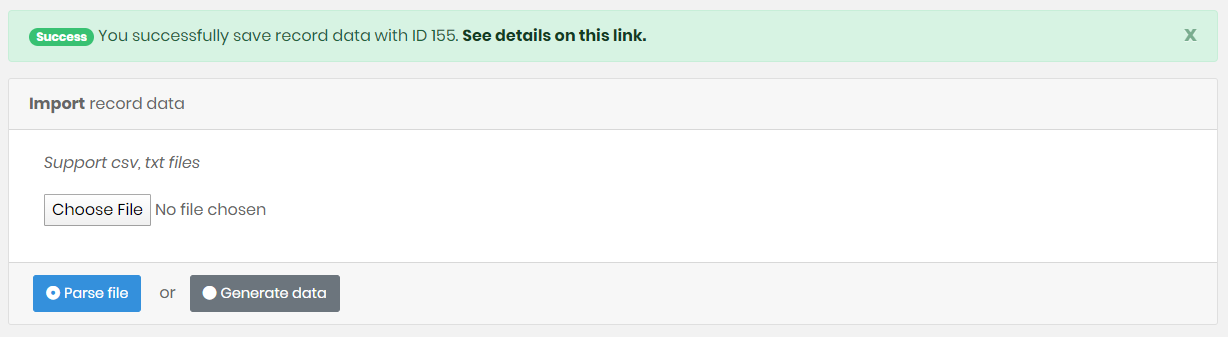
\includegraphics[width=\textwidth]{slike/import_success.png}
\end{center}
\caption{Primer sporočila, ki se pojavi po uspešno shranjeni meritvi. Odebeljeni del sporočila omogoča prehod do strani z analizo uvožene ali generirane meritve.}
\label{ss-import-success}
\end{figure}

V primeru, da pri uvozu meritve uporabnik izbere napačen format datoteke, se po kliku na gumb \sn{Parse file} izpiše rdeče opozorilo z besedilom \sn{File is not in proper format.} (slika~\ref{ss-import-error}).

\begin{figure}[h]
\begin{center}
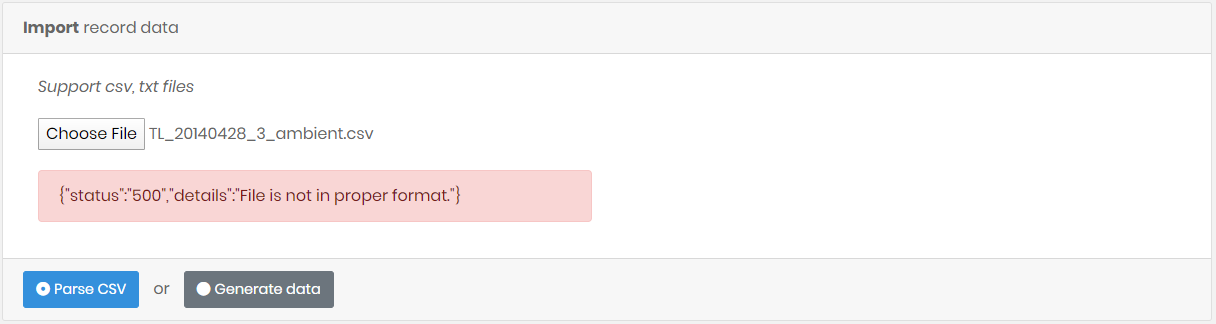
\includegraphics[width=\textwidth]{slike/import_error.png}
\end{center}
\caption{Opozorilo v primeru napačnega formata datoteke pri uvozu meritve.}
\label{ss-import-error}
\end{figure}


\section{Pregled, iskanje in filtriranje meritev}

Glavna funkcionalnost v spletni aplikaciji predstavlja pregled podrobnosti in vizualizacija z grafično analizo meritve. V njej prikažemo uvožene, izračunane, ugotovljene in predvidene podatke o izbrani meritvi v obliki alinej, tabel ali grafov. 

Najprej izpišemo podatke iz datoteke, predstavimo tudi robne vrednosti, kot prikazuje slika~\ref{ss-record-page} v spodnjem delu desno.
Robne vrednosti so zapisane v obliki tabele in določajo:
\begin{itemize}
	\item Limits – oznaka vrednosti, Value – dejanska vrednost, Count – število ponovitev,
	\item Min T (°C) – najnižja temperaturna vrednost,
	\item Max T (°C) – najvišja temperaturna vrednost,
	\item Min RH (\%) – najnižja vrednost relativne vlage,
	\item Max RH (\%) – najvišja vrednost relativne vlage.
\end{itemize}


Levi del slike prikazuje ime osebe in čas od uvoza ter komentar meritve.

\begin{figure}[h]
\begin{center}
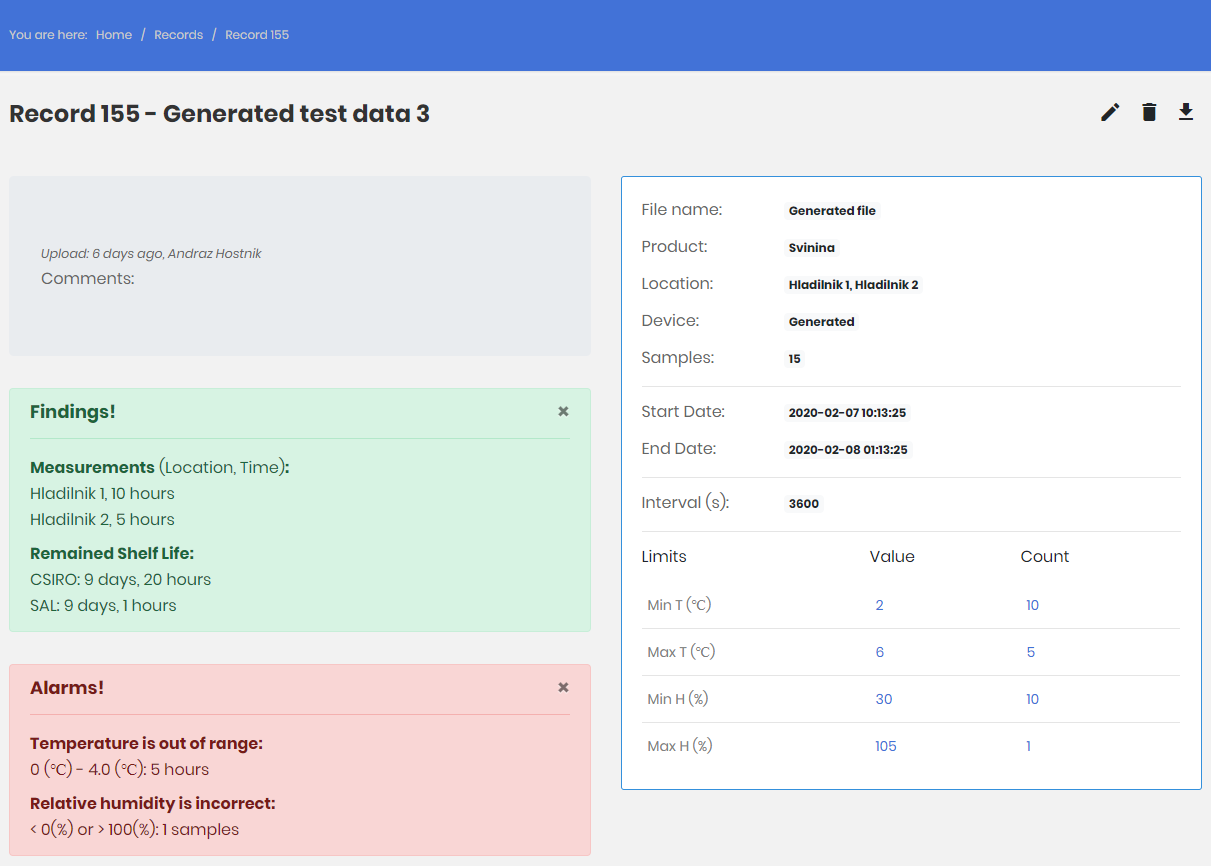
\includegraphics[width=\textwidth]{slike/record_page_11.png}
\end{center}
\caption{Del zaslonskega posnetka strani z analizo in podrobnosti meritve.}
\label{ss-record-page}
\end{figure}

Na zeleni podlagi so izpisane splošne ugotovitve hladne verige iz podatkov. Podatek \sn{Measurements (Location, Time)} prikazuje čas meritve na posamezni lokaciji. Čas je zapisan v človeku berljivem načinu. Iz slike~\ref{ss-record-page} lahko izberemo, da je meritev bila izvedena na dveh lokacijah, in sicer Hladilnik 1 s časom 10 ur ter Hladilnik 2 s časom 5 ur. 

Spodaj je primer izvorne kode za izpis skupnega časa po lokacijah meritve. Metoda \verb=forHumans= je del knjižnice Carbon, ki služi kot razširitev programskemu jeziku PHP pri uporabi s časom (ang. DateTime) \cite{carbon-framework}:

\begin{lstlisting}[language=PHP, style=mystyle]
<div class="alert alert-success" role="alert">
    <h4 class="alert-heading">Findings!</h4>
    <p><b>Measurements</b> (Location, Time):</p>
    @foreach($locationsPerTime as $location)
    <p>{{ $location->name }}, {{ $location->sumTime->forHumans() }}</p>
    @endforeach
</div>
\end{lstlisting}

\clearpage

Pod izpisom skupnega časa po lokacijah se izpiše podatek o preostali dobi uporabnosti živila po modelu CSIRO in modelu SAL. Podrobno o omenjenih dveh podatkih je opisano v naslednjem poglavju.

V primeru, da meritev vsebuje opozorila, se nam le-ta izpišejo na rdeči podlagi. Podatek \sn{Temperature is out of range} kot območje prikaže čas pri katerem je bilo živilo izven priporočenih temperatur hranjenja. V primeru na sliki~\ref{ss-record-page} razberemo, da je bilo živilo 5 ur izven priporočenega območja temperature (od 0 °C do 4 °C). 
Če meritev vsebuje neveljavne vrednosti relativne vlage, izpišemo število takih vzorcev pri podatku \sn{Relative humidity is incorrect}. Na sliki~\ref{ss-record-page} vidimo, da je en vzorec meritve vseboval vrednost manjšo od 0 \% ali večjo od 100 \%.


\begin{figure}[h]
\begin{center}
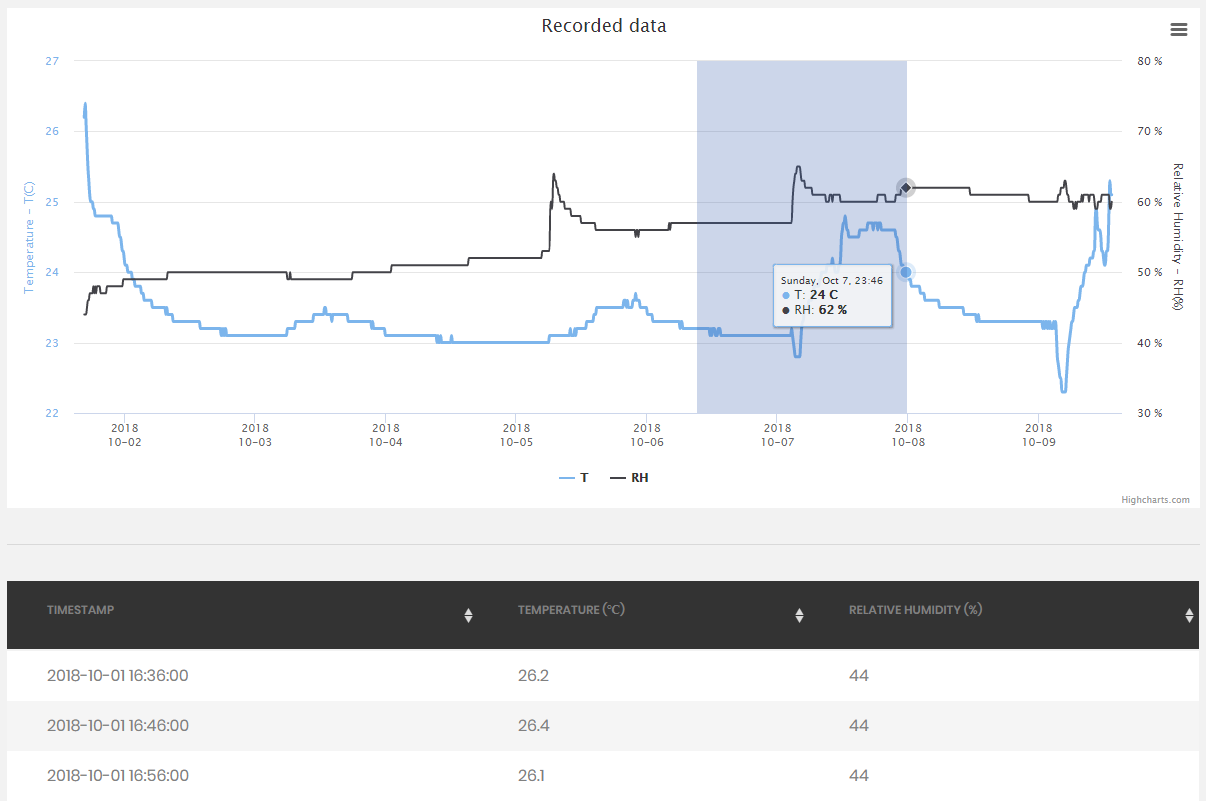
\includegraphics[width=\textwidth]{slike/record_page_2_zoom.png}
\end{center}
\caption{Graf in tabela prikaza meritvenih podatkov.}
\label{ss-record-page-zoom}
\end{figure}

V osrednjem delu strani s podrobnostjo meritve se nahaja graf, ki prikazuje podatke o temperaturi in relativni vlagi v odvisnosti od časa. Za grafom je prikazan tudi izpis omenjenih podatkov v obliki tabele.
Na sliki~\ref{ss-record-page-zoom} vidimo, da smo označili časovni interval, ki ga želimo povečati. Z miško smo se ustavili na vrednosti, ki je prikazana v malem pojavnem oknu (čas 23:46, temperatura 24 °C, relativna vlaga 62 \%). V primeru, da želimo večjo preglednost, lahko s klikom na posamezno postavko v agendi na dnu grafa skrijemo vrednosti označene postavke.  


\section{Napoved preostale dobe uporabnosti izbranega živila}

V aplikaciji smo za izračun dobe uporabnosti živila implementirali modela, ki sta opisana v poglavju \ref{modela-za-izracun-sl}.


Funkciji za izračun preostale dobe uporabnosti živila po modelu CSIRO in SAL:

\begin{lstlisting}[language=PHP, style=mystyle]
// izracun za model CISRO
public function getSl_CSIRO($sl, $interval, $temperature){

    $t = $interval / 86400; // v casu t
    $k = pow(1 + round($temperature) * 0.1, 2); // koeficient
    return ($sl - $t * $k); // preostala doba uporabnosti
}
// izracun za model SAL
public function getSl_SAL($sl, $sl_ref, $interval, $temperature){

    $t = $interval / 86400; // v casu t
    $t_sal = $this->getT_SALfromTable( round($temperature) ); // doba uporabnosti pri temperaturi T prebrana iz tabele SAL
    $k = $sl_ref / $t_sal; // koeficient iz referencne dobe uporabnosti deljeno z $t_sal
    return ($sl - $t * $k); // preostala doba uporabnosti
}
\end{lstlisting}

Za vsak zapis meritve kličemo zgornji funkciji s parametri preostale dobe uporabnosti (\verb=$sl=), interval beleženja (\verb=$interval=) in vrednost temperature (\verb=$temperature=). Pri modelu SAL dodatno še parameter referenčne dobe uporabnosti (\verb=$sl_ref=). Rezultat vsake funkcije je preostala doba uporabnosti.

\begin{figure}[h]
\begin{center}
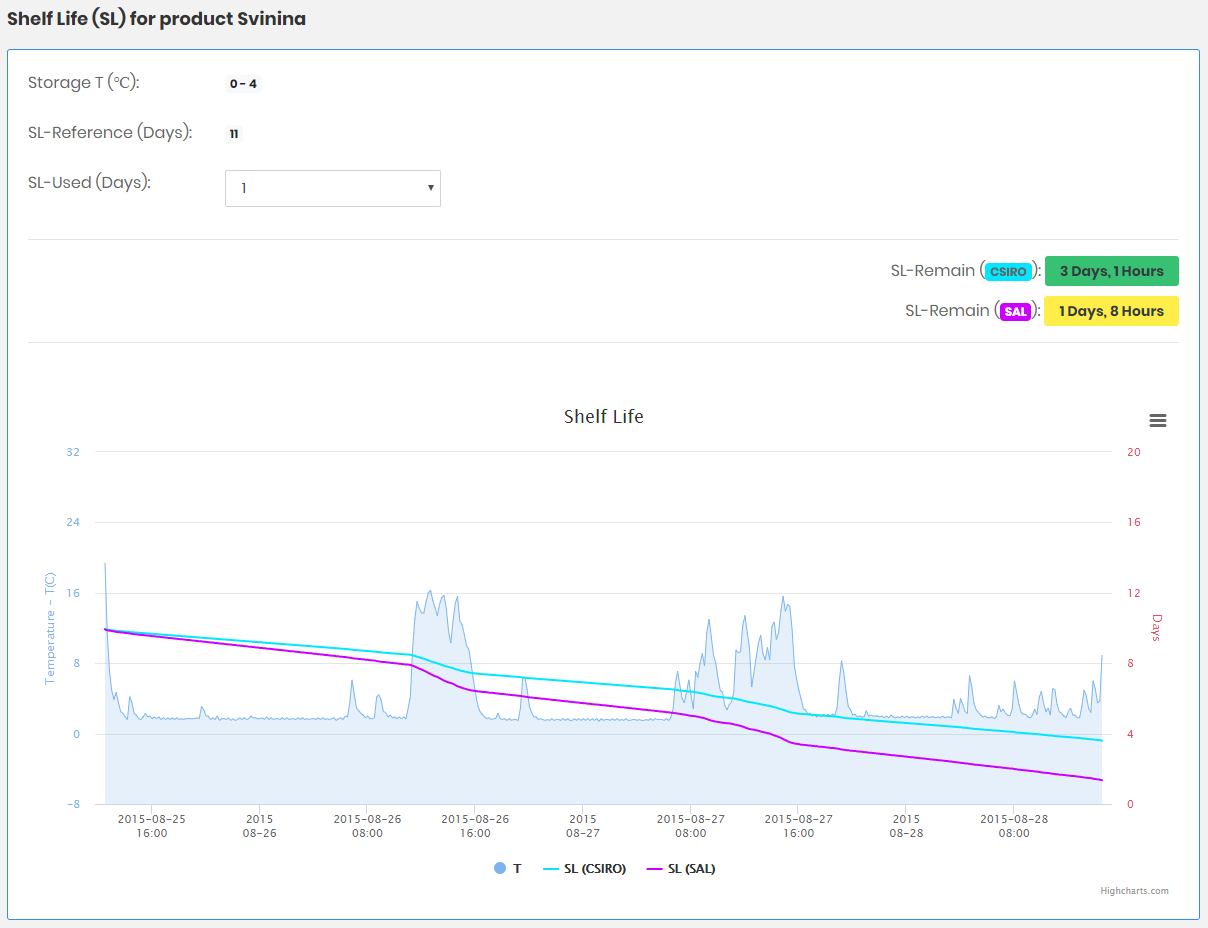
\includegraphics[width=\textwidth]{slike/record_page_333.png}
\end{center}
\caption{Zaslonski posnetek s podatki in grafom dobe uporabnosti.}
\label{ss-record-page-sl}
\end{figure}

Na sliki~\ref{ss-record-page-sl} v zgornjem odseku zaslonskega posnetka vidimo, da se graf dobe uporabnosti nanaša na živilo svinina (\sn{Shelf Life (SL) for product Svinina}), ki ima priporočeno temperaturo hranjenja med 0 in 4 °C (\sn{Storage T (°C)}) in referenčno dobo uporabnosti 11 dni (\sn{SL-Reference (Days)}).

Iz spustnega seznama smo izbrali, da je pred meritvijo minil en dan od takrat, ko smo meso pričeli spremljati in beležiti meritve. V tem primeru to pomeni, da predpostavljamo, da je bila svinina hranjena v območju priporočenih temperatur (\sn{SL-Used (Days)}).

Na grafu modro obarvano območje prikazuje temperaturo, turkizno modra črta dobo uporabnosti po modelu CSIRO in vijoličasta črta dobo uporabnosti po modelu SAL v odvisnosti od časa (x os na grafu).

Iz zgornjega primera lahko razberemo, da je doba uporabnosti živila vseskozi padala linearno navzdol. Pri vrednosti temperature približno 16 ºC je padala hitreje kot običajno. Doba uporabnosti pri modelu SAL je tam znašala nekoliko manj kot za model CSIRO.

Na koncu meritve pa je preostala doba uporabnosti znašala 3 dni in 1 uro za model CSIRO in 1 dan 8 ur za model SAL (\sn{SL-Remain}).



\section{Pregled in urejanje živil}

Do strani z nastavitvami (\sn{Settings}) imajo dostop uporabniki z vlogo administrator ali urednik. Na omenjeni strani je v prvem razdelku pregled vseh živil v obliki tabele (\sn{Products}). Uporabniki imajo možnost dodajanja, urejanja ali brisanja živil.

\begin{figure}[h]
\begin{center}
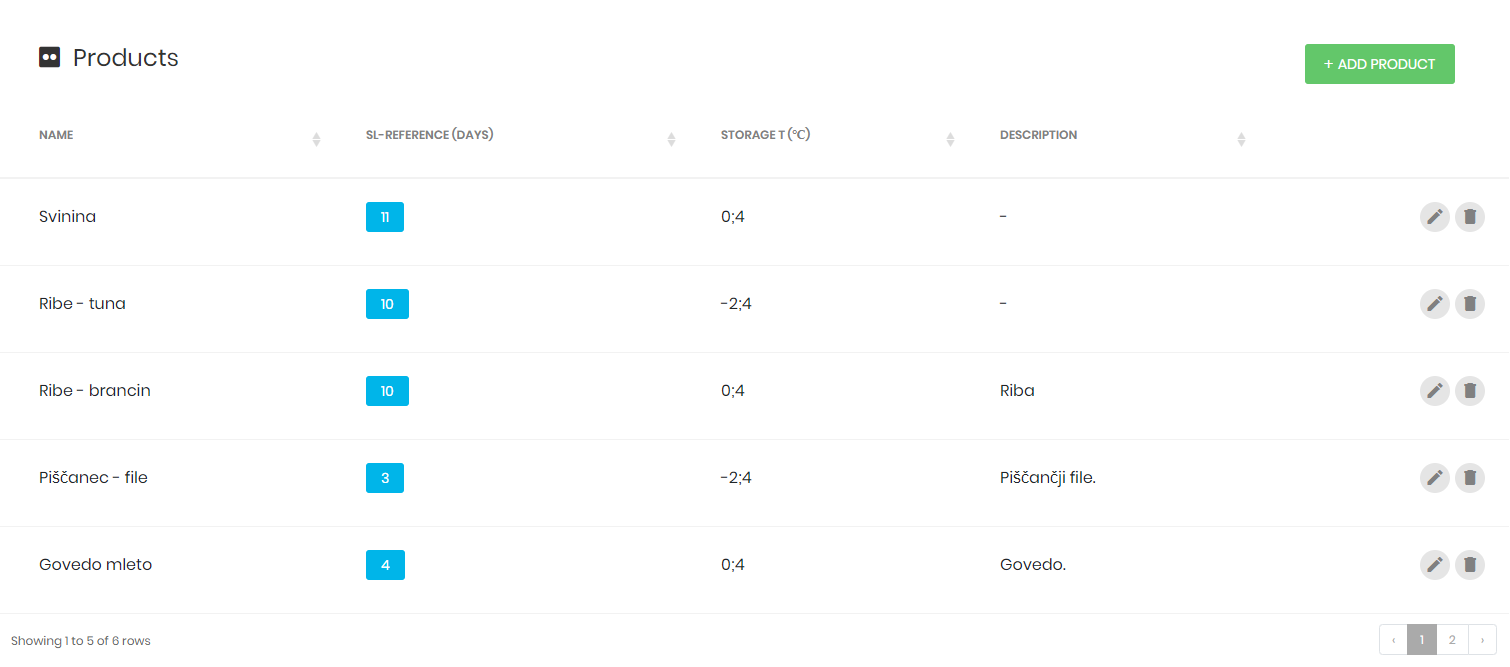
\includegraphics[width=0.9\textwidth]{slike/products.png}
\end{center}
\caption{Na sliki so prikazana živila, ki smo jih predhodno vnesli v aplikacijo v razdelku (\sn{Products}).}
\label{ss-settings-products}
\end{figure}

Na sliki~\ref{ss-settings-products} je v prvem stolpcu definirano ime (\sn{Name}), v drugem referenčna doba uporabnosti v dnevih (\sn{SL-Reference (Days)}), v tretjem območje priporočene temperature hranjenja (\sn{Storage T (°C)}) in v zadnjem opis živila. Z modro barvo smo odebelili pomembnejše informacije. Na koncu vsake vrstice se nahajata ikoni za urejanje in brisanje živila.



\section{Pregled in urejanje lokacij}

V tabelaričnem pogledu so na strani z nastavitvami (\sn{Settings}) v drugem razdelku prikazane vse lokacije v aplikaciji (\sn{Locations}). Uporabniki imajo možnost pregleda, urejanja ter dodajanja novih lokacij (slika~\ref{ss-settings-location}).


\begin{figure}[h]
\begin{center}
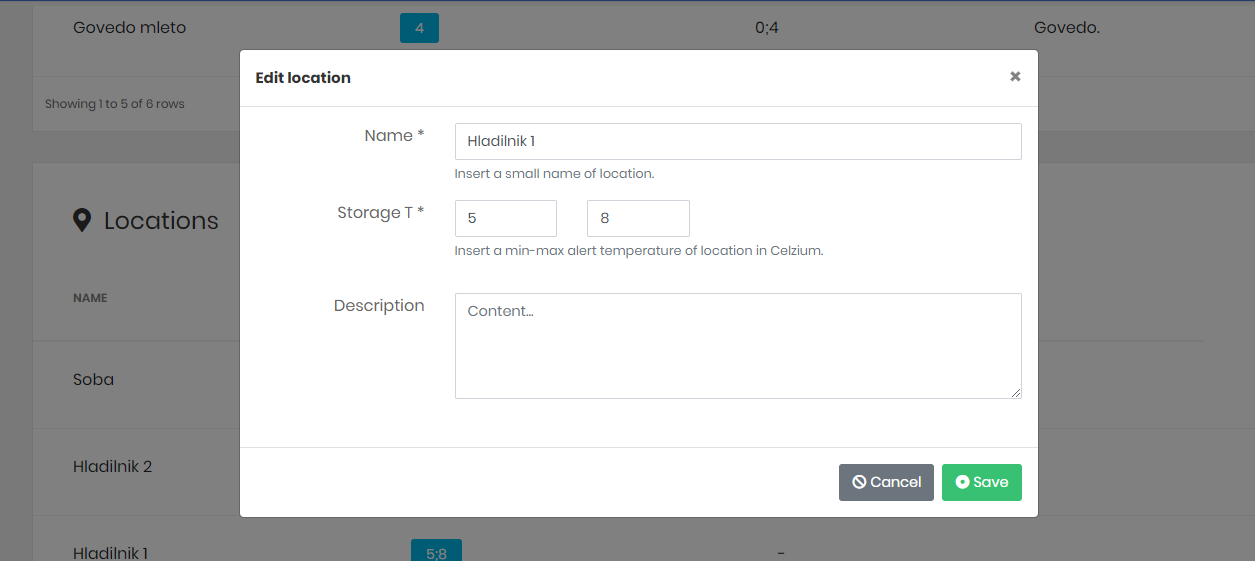
\includegraphics[width=0.9\textwidth]{slike/location_edit.png}
\end{center}
\caption{Primer dialoga za urejanje lokacije.}
\label{ss-settings-location}
\end{figure}

Dialog iz slike~\ref{ss-settings-location} odpremo s klikom na ikono za urejanje pri posamezni lokaciji. Spreminjamo lahko podatke kot so ime (\sn{Name*}), območje delovne temperature (\sn{Storage T*}) in opcijsko opis lokacije. S klikom na gumb shrani (\sn{Save}) se zapre dialog in prikaže besedilo o uspešnosti shranitve.


\clearpage


\section{Pregled senzorskih naprav}

V aplikaciji smo pri uvozu meritev upoštevali dva različna formata datoteke, ki sta rezultat meritvenih naprav TIDA \cite{dialoger-tida} in RHT10 \cite{rht10-dialogger}.

Tretji format smo določili za potrebe simulacije pogojev hladne verige in testiranja. Zaradi ročno ustvarjenih podatkov smo ta tip naprave poimenovali kar 'Generated'.
Tako imamo v aplikaciji podprte naslednje tri tipe naprav: TIDA, RHT10 in Generated (slika~\ref{ss-settings-devices}).

\begin{figure}[h]
\begin{center}
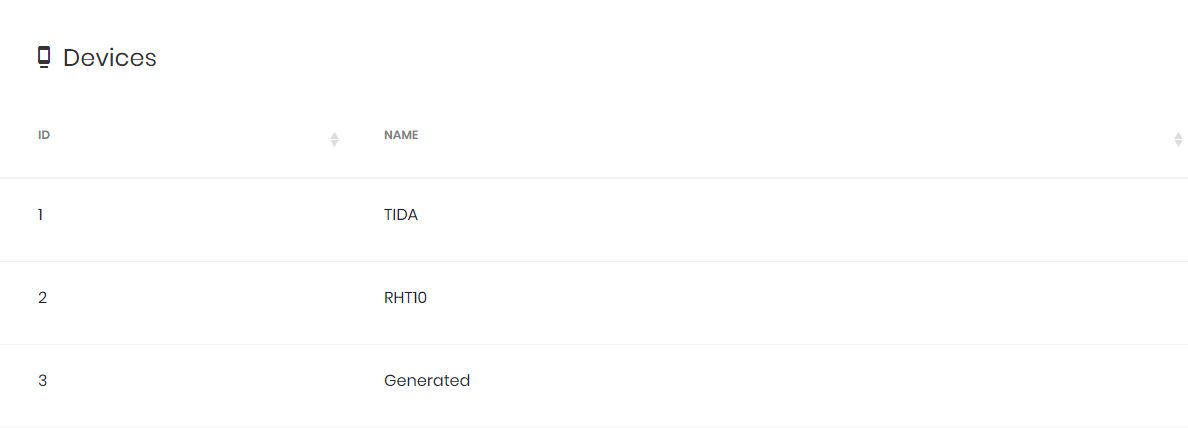
\includegraphics[width=\textwidth]{slike/devices.png}
\end{center}
\caption{Na strani z nastavitvami imamo pregled senzorskih naprav (\sn{Devices}).}
\label{ss-settings-devices}
\end{figure}


\clearpage


\section{Pregled in potrditev uporabnikov}

Administrator ima možnost pregleda in odobritve uporabnikov na strani z nastavitvami v razdelku \sn{User data}. V prvem stolpcu sta izpisana ime in e-pošta, v drugem vloga in v tretjem gumb za potrditev (\sn{Approve}) ali čas potrditve v primeru, da uporabnik že ima dostop (slika~\ref{ss-settings-users}).

\begin{figure}[h]
\begin{center}
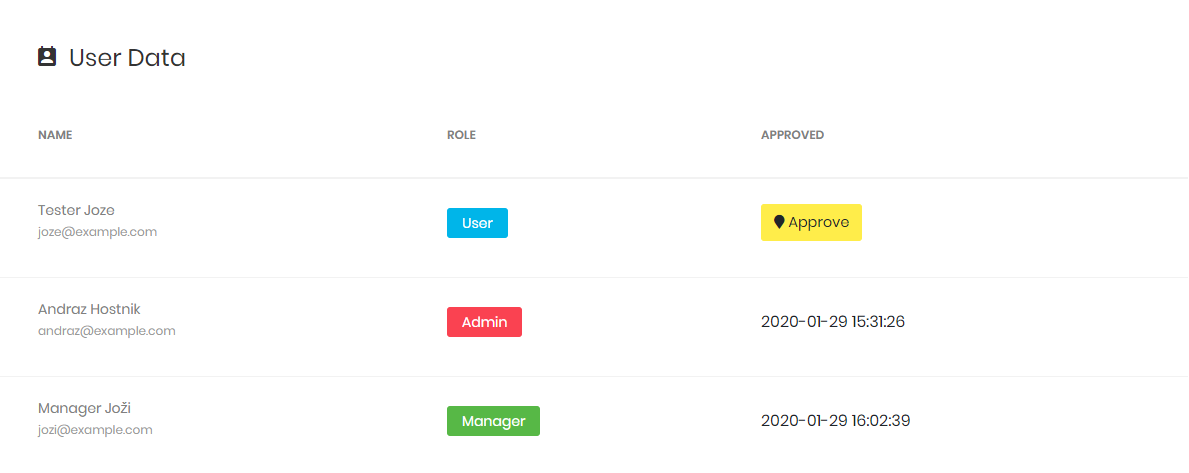
\includegraphics[width=\textwidth]{slike/users.png}
\end{center}
\caption{Pregled uporabnikov, njihovih vlog in status potrditve.}
\label{ss-settings-users}
\end{figure}



\chapter{Testiranje}
\label{testiranje}

Spletno aplikacijo smo najprej testirali v lokalnem okolju, kjer smo tudi razvijali nove funkcionalnosti. Kasneje smo spletno aplikacijo, vključno s podatkovno bazo in testnimi podatki, prenesli na zakupljeno gostovanje.

\section{Testiranje spletne storitve}

Pri testiranju smo si pomagali z orodjem za razvijalce, ki je del brskalnika Google Chroome (\sn{DevTools}). V njem smo preverjali zapis kode HTML in posamezne klice spletnih storitev \cite{google-devtools}.

Testirali smo tudi s pomočjo paketa Dump Server, ki je del ogrodja Laravel. Omenjeni paket nam v ozadju delovanja aplikacije zbira podatke, ki smo jih v izvorni kodi določili za pošiljanje preko funkcije \verb=dump()=, in izpis preko ukazne vrstice \cite{laravel-dump}.

Za vsebinsko testiranje meritev pa smo razvili posebno funkcionalnost. Simulirali smo podatke, ki jih vsebujejo meritvene datoteke preko generatorja podatkov, ki je bil podrobneje opisan v poglavju \ref{uvoz-in-generiranje-meritev}.


\section{Postavitev aplikacije na testno okolje}

Spletno aplikacijo smo prenesli na javno dostopno gostovanje z namenom, da jo lahko analizirajo tudi drugi uporabniki.

Najprej smo v administrativnem vmesniku ponudnika gostovanja kreirali podatkovno bazo, kjer smo z pomočjo orodja \verb=phpMyAdmin= \cite{phpmyadmin-framework} uvozili podatkovno shemo in podatke iz lokalnega okolja (slika~\ref{ss-admim-gui}). Za tem smo preko protokola za prenos datotek (FTP) prenesli še ostale datoteke spletne strani.

\begin{figure}[h]
\begin{center}
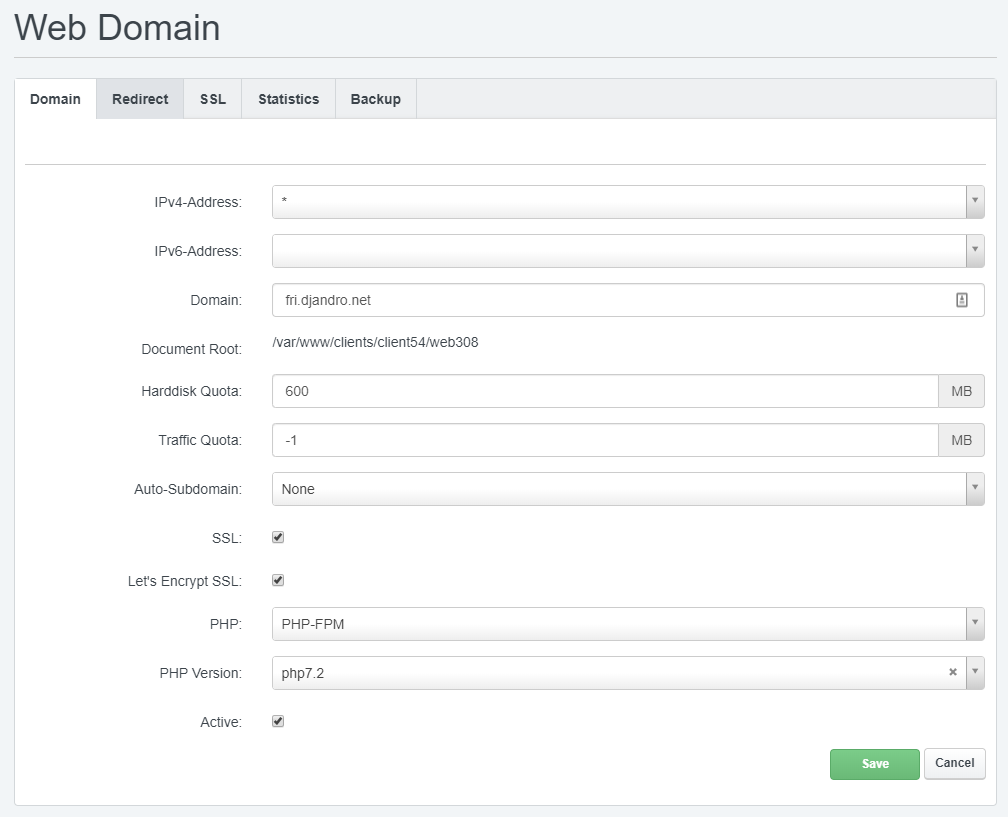
\includegraphics[width=\textwidth]{slike/admin_vmesnik.png}
\end{center}
\caption{Administrativni vmesnik ponudnika gostovanja.}
\label{ss-admim-gui}
\end{figure}



\chapter{Sklepne ugotovitve}

V diplomskem delu smo razvili spletno aplikacijo za vnos, shranjevanje, analizo in vizualizacijo podatkov iz hladne verige. Za podatke, ki so v različnih podatkovnih formatih, smo uspešno razvili enoten uvoz podatkov z možnostjo konfiguracije posameznih senzorskih meritev. Razvili smo generator podatkov, ki pomaga uporabnikom pri ustvarjanju podatkov v simuliranih pogojih hladne verige za potrebe optimizacije procesa, hkrati pa nam je bil v pomoč pri samem testiranju aplikacije. 

Osrednja funkcionalnost aplikacije je pregled nad posamezno meritvijo, kjer uporabniku podrobno analiziramo in vizualiziramo ključne podatke ter po modelu CSIRO in SAL napovemo preostalo dobo uporabnosti. Izpostavili bi še nekaj funkcionalnosti, ki uporabnikom olajšajo uporabo aplikacije:

\begin{itemize}
	\item omogočanje prijave, odjave, registracije in potrditve uporabnika,
	\item tri uporabniške vloge glede na tip uporabe (administrator, urednik, obiskovalec),
	\item možnost spreminjanja števila dni med meritvijo in izvora živila,
	\item iskanje in filtriranje meritev,
	\item dodajanje, urejanje in brisanje živil,
	\item dodajanje, urejanje in brisanje lokacij.
\end{itemize}

Z izbiro ogrodja Laravel in spletne predloge HTML smo pohitrili razvoj, saj so bili osnovni spletni gradniki in grafične komponente že del omenjenih dveh ogrodij.


Naša spletna aplikacija uspešno rešuje zgoraj omenjene probleme iz področja senzorskih meritev hladne verige. Vidimo pa še kar nekaj možnosti za razširitev in uvedbo na omenjenem področju. Smiselno bi bilo nadaljevati z razvojem in razširiti trenutne funkcionalnosti z naslednjimi:

\begin{itemize}
	\item poleg ročnega uvoza meritev bi lahko imela aplikacija povezavo z ostalimi podatkovnimi bazami ali spletnimi storitvami s področja hladne verige,

	\item pri dobi uporabnosti živila, bi lahko aplikacija sama preračunala preostalo dobo uporabnosti glede na trenutni dan ogleda meritve,

	\item pri napovedovanju preostale dobe uporabnosti živila bi lahko upoštevali še mikrobiološke podatke živila,

	\item pri analizi meritve, bi lahko sistem sam ugotovil različne lokacije, glede na izmerjene vrednosti temperatur,

	\item na grafu meritve bi lahko prikazali še območje priporočene temperature hranjenja živila,

	\item dodali bi urejanje uporabniških podatkov kot so: ime, priimek in e-pošta.
\end{itemize}



% \newpage %dodaj po potrebi, da bo številka strani za Literaturo v Kazalu pravilna!
\ \\
\clearpage
\addcontentsline{toc}{chapter}{Literatura}
\bibliographystyle{plain}
\bibliography{literatura}


\end{document}

